\documentclass{thesis-umich}
\usepackage[section]{placeins}

\author{Colin Tinsman}
\committee{
Dr. Lu Li, \\
Dr. Cagliyan Kurdak \\
Dr. Kai Sun \\
Dr. Zhaohui Zhong
}
\department{Applied Physics}
\title{Thermal Hall Effect Measurements using Strontium Titanate Microthermometers}
\year=2019

\acknowledgments[2]{I would like to thank Ctirad Uher for providing the bismuth crystals, as well as Sara Haravifard for providing the strontium copper borate samples.}


\begin{document}

\doublespacing

\chapter{The Thermal Hall Effect}


\section{Thermal Hall Conductivity in General}

The thermal Hall effect is the thermal analogue of the much more well known
(electrical) Hall effect. As the Hall effect can be understood as generalizing
the electrical conductivity \(\sigma\) to a tensor in Ohm's law: \[\mathbf{j} =
	\sigma \mathbf{E} \Rightarrow \begin{pmatrix} j_x \\ j_y \end{pmatrix}
= \begin{pmatrix} \sigma_{xx} & \sigma_{xy} \\ -\sigma_{xy} & \sigma_{yy}
\end{pmatrix} \begin{pmatrix} E_x \\ E_y \end{pmatrix} \] The thermal Hall
effect generalizes the thermal conductivity \(\kappa\) to a tensor in Fourier's
law: \[\mathbf{q} = -\kappa \nabla u \Rightarrow \begin{pmatrix} q_x \\ q_y
	\end{pmatrix} = -\begin{pmatrix} \kappa_{xx} & \kappa_{xy} \\
		-\kappa_{xy} & \kappa_{yy} \end{pmatrix} \begin{pmatrix}
		\partial_x u \\ \partial_y u \end{pmatrix} \] where \(u\) is
	the temperature field and \(\mathbf{q}\) is the heat current. Before
	discussing the origin of of the thermal Hall conductivity
	\(\kappa_{xy}\), we should establish how heat flows through such a
	material. Let's assume we have an isotropic material (i.e.
	\(\kappa_{xx} = \kappa_{yy}\)). The conductivity tensor can be
	rewritten as \[\begin{pmatrix} \kappa_{xx} & \kappa_{xy} \\
			-\kappa_{xy} & \kappa_{xx} \end{pmatrix} = \kappa_{xx}
		\begin{pmatrix} 1 & \kappa_{xy}/\kappa_{xx} \\
		-\kappa_{xy}/\kappa_{xx} & 1 \end{pmatrix} = \kappa_{xx}
\begin{pmatrix} 1 & \tan \theta_H \\ -\tan \theta_H & 1 \end{pmatrix} \] where
\(\theta_H = \arctan \kappa_{xy}/\kappa_{xx}\) is the definition of the thermal
Hall angle. Writing down the Heat equation, and splitting the conductivity into
its symmetric and antisymmetric parts: \begin{align*} -\nabla \cdot \mathbf{q}
	= c \rho \partial_t u = \nabla \cdot (\kappa \nabla u) &= \nabla \cdot
	(\kappa_{xx}(\mathbb{I} + \kappa_{\mathrm{antisym}}) \nabla u) \\ &=
	\kappa_{xx}\nabla^2 u + \kappa_{xx}\nabla \cdot
	(\kappa_{\mathrm{antisym}} \nabla u) \end{align*} where c is the heat
capacity and \(\rho\) is the mass density. Writing out the
\(\kappa_\mathrm{antisym}\) term explicitly:
\begin{align*}\begin{pmatrix} \partial_x & \partial_y \end{pmatrix} \begin{pmatrix} 0 & \tan
\theta_H \\ -\tan \theta_H & 0 \end{pmatrix} \begin{pmatrix} \partial_x u \\
\partial_y u \end{pmatrix} &= \begin{pmatrix} \partial_x & \partial_y
\end{pmatrix} \begin{pmatrix} \tan \theta_H \partial_x u \\ -\tan \theta_H
\partial_y u \end{pmatrix} \\ &= \tan \theta_H \partial_{xy} u - \tan \theta_H
\partial_{xy} u = 0\end{align*} Thus the equation reduces to the
isotropic heat equation,
\(c\rho \partial_t u = \kappa_{xx} \nabla^2 u\)! Thus, it might seem
like the thermal Hall conductivity would have no effect on the flow of
heat through the material. Indeed, when studying the heat equation, the
conductivity tensor \(\kappa\) is usually assumed to be symmetric.
However, if we impose the Neumann boundary condition
\(g = -\hat{n} \cdot \mathbf{q}\) for some known function \(g\), the
effect of the thermal Hall conductivity can be seen:
\begin{align*}-\hat{n} \cdot \mathbf{q} &= \hat{n} \cdot \kappa \nabla u \\
&= \kappa_{xx} \begin{pmatrix} n_x & n_y \end{pmatrix} \begin{pmatrix} 1 & \tan
\theta_H \\ -\tan \theta_H & 1 \end{pmatrix} \begin{pmatrix} \partial_x u \\
\partial_y u \end{pmatrix} \\ &= \kappa_{xx} \begin{pmatrix} n_x & n_y
\end{pmatrix} \begin{pmatrix} \partial_x u + \tan \theta_H \partial_y u \\
-\tan \theta_H \partial_x u + \partial_y u \end{pmatrix} \\ &= \kappa_{xx} n_x
(\partial_x u + \tan \theta_H \partial_y u) + \kappa_{xx} n_y (-\tan \theta_H
\partial_x u + \partial_y u)  \end{align*} Taking for example
\(\hat{n} = (1, 0)\) and \(g = 0\) (perfectly insulating boundary
conditions):
\[ 0 = - \hat{n} \cdot \mathbf{q} = \kappa_{xx} (\partial_x u + \tan \theta_H
\partial_y u) \Rightarrow \partial_x u = -\tan \theta_H \partial_y u\]
In general, the derivative normal to the boundary is specified in terms
of the transverse derivative and the thermal Hall angle.

In order to see what this kind of boundary condition does in practice,
we can simulate a material with a thermal Hall coefficent using the
finite element method. For simplicity, we will look first at steady
state solutions (i.e.~those with \(\partial_t u = 0\)). Thus we will
need to solve the elliptic partial differential equation
\(-\nabla \cdot (\kappa \nabla u) = 0\). We start by expressing this
equation in weak form by multiplying it by a test function \(v\) and
integrating over the function's domain \(\Omega\):
\[ -\nabla \cdot (\kappa \nabla u) = 0 \Rightarrow -\int_\Omega \nabla \cdot
(\kappa \nabla u) v dx = 0 \] The function \(u(x,y)\) is said to solve
the weak problem if this equation holds for all functions \(v(x,y)\),
where \(v(x, y) = 0\) anywhere we have specified \(u\) on the boundary
(i.e.~imposed Dirichlet boundary conditions). By integrating by parts,
this becomes:
\[ - \int_\Omega \nabla \cdot (\kappa \nabla u) v dx = \int_\Omega \kappa \nabla
u \cdot \nabla v dx - \int_{\partial \Omega} (\hat{n} \cdot \kappa\nabla u) v ds\]
where the second integral on the right hand side is over the boundary of
\(\Omega\). The second integral can be rewritten in terms of the Neumann
boundary condition:
\[ - \int_{\partial\Omega} (\hat{n} \cdot \kappa \nabla u) v ds =
\int_{\partial\Omega} g v ds\] and so we have cast the problem in a form
suitable for solving with the finite element method, in terms of the
bilinear form
\[ a(u, v) = \int_\Omega \kappa \nabla u \cdot \nabla v dx \] and the
linear form \[ L(v) = -\int_{\partial \Omega} g v ds \] as
\(a(u, v) = L(v)\). By discretizing the problem using standard methods
over a suitable mesh, the problem reduces to solving a linear system.
There are many references which go into detail on finite element
analysis, but I used \cite{LangtangenLogg2017} which covered the
specific Python library I used to run the following simulations.

\begin{figure}
\centering
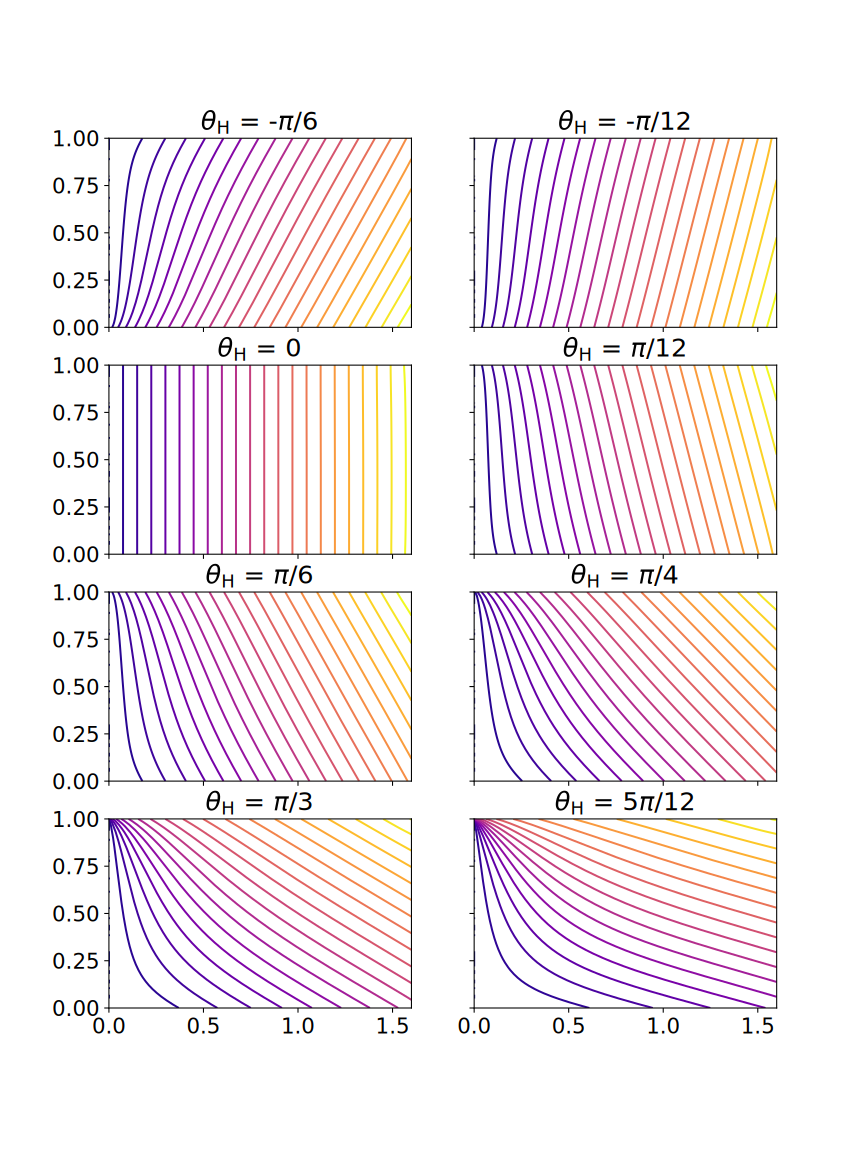
\includegraphics[width=\textwidth]{figures/thall_isotherm.pdf}
\caption[Thermal Hall Isotherms]{Thermal Hall Isotherms. The left side of each simulation is
held to \(T=0\), the right has a heater with unit power, and the upper
and lower edges are insulating.\label{thall_iso}}
\end{figure}

\begin{figure}
\centering
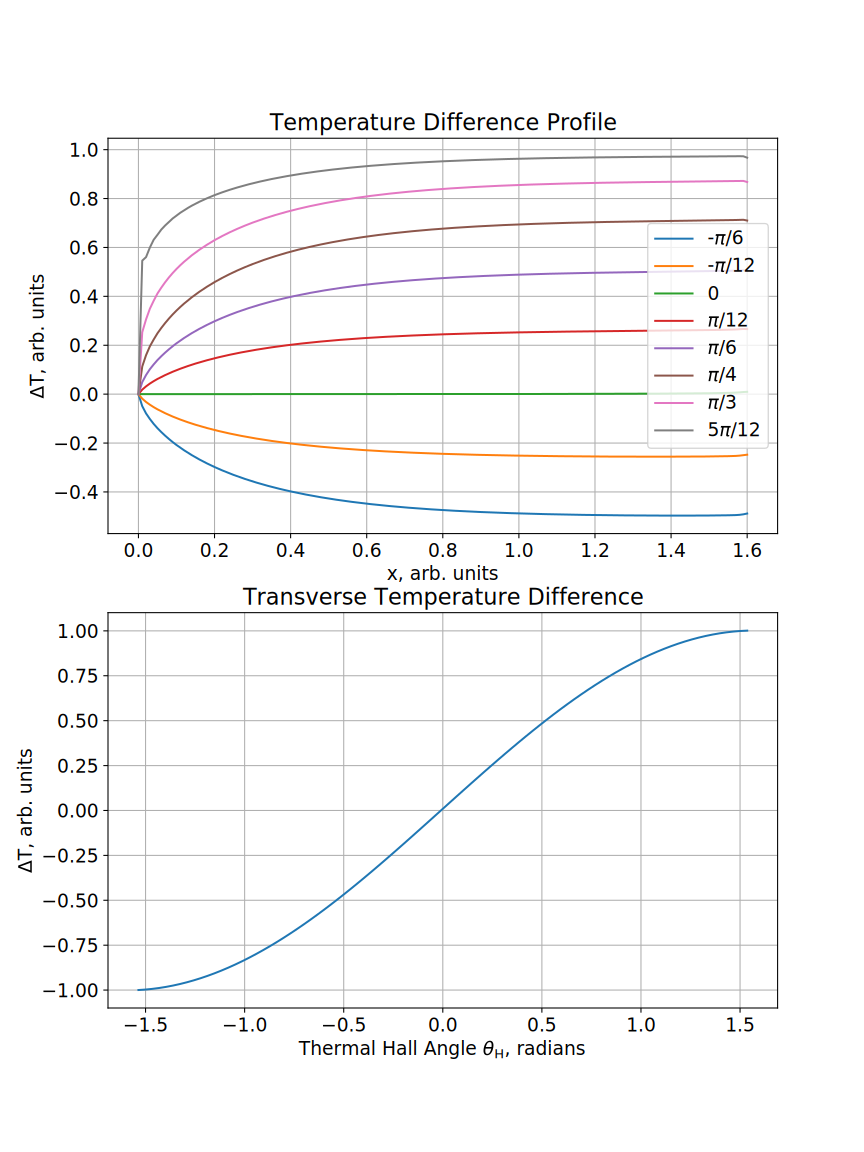
\includegraphics[width=0.9\textwidth]{figures/thall_profile.pdf}
\caption[Thermal Hall Temperature Profiles]{Thermal Hall Temperature Profiles. Top: Temperature difference across
	the sample transverse to the applied heat (y axis in figure
	\ref{thall_iso}) at different points along the sample for different
	thermal Hall angles. Note that for each angle, the temperature
	difference approaches a constant value far from the cold finger.
	Bottom: The same temperature difference at a fixed position as a
function of the thermal Hall angle. Note that for experimentally relevant values of the thermal Hall angle (\(\theta_H \approx 1^\circ\)), \(\Delta T\) is proportional to \(\theta_H\).   \label{thall_prof}}
\end{figure}

This dependence of the Hall signal on the particular boundary condition should
not be suprising to anyone who is experienced making electrical transport
measurements. Indeed, DC electrical transport can be modeled using an analogous
partial differential equation \[ \nabla \cdot (\sigma \nabla V) = 0 \] where
$V$ is the electric potential and $\sigma$ is the conductivity tensor. The
typical geometry for a (non-thermal) Hall effect measurement involves measuring
the voltage at four points on the sample, with the edges of the sample
electically insulating. This gives us the same Neumann boundary condition as
before, via Ohm's law rather than Fourier's law: \[ \hat{n} \cdot \mathbf{j} =
\hat{n} \cdot \sigma \nabla V = 0\] where $\mathbf{i}$ is the current density.
If instead we wish to eliminate the effect of the Hall conductivity, a
different geometry known as a Corbino disk is used~\cite{Eo2018}. This geometry consists of
two large electrodes in the shape of concentric rings, leaving an annular
region where current flows through the sample of interest. In effect, this
clamps the voltage at each point on the two rings (to values which depend on
the applied current and the conductivity of the sample), effectively giving us
a Dirichlet boundary condition (i.e. specifing the voltage) at every point on the boundary. This supresses
the effect of the Hall conductivity, and thus this type of of measurement is
good for isolating the magnetoresistance of a sample.

\begin{figure} \centering
	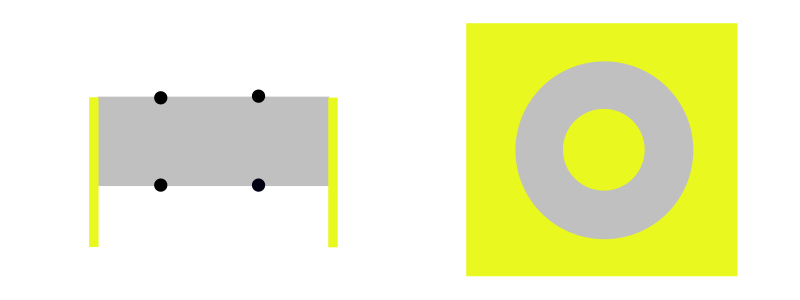
\includegraphics[width=\textwidth]{figures/ehall_geometry.pdf}
	\caption[Electrical Transport Geometries]{Electrical Transport
	Geometries. Left: Hall bar geometry. Current is fed in through the gold
contacts on the left and right, and the voltage measured at the black points.
The upper and lower boundaries are insulating. Right: Corbino disk. The voltage
is measured between the inner and outer contacts (gold). Since there is no
insulating boundary, the Hall conductivity is suppressed.} \end{figure}

This analogy between thermal and electrical transport begs the question: Could
one measure thermal conductivity with a ``thermal Corbino disk''? Maybe, but in
practice it would never be necessary for a very simple reason: in real
materials, the thermal Hall angle is rarely more than a few degrees. Table
\ref{hallAngleTable} lists a few selected thermal Hall angles reported in the
literature. In all of these materials, the thermal Hall conductivity is the
result of some kind of (quasi-)particle excitation. In the next section, we
will discuss the thermal Hall conductivity of electrons in metals. However, the
last two entries in the table list thermal Hall conductivities which are the
result of excitations which carry spin but not charge. It is this kind of
experiment where measurements of the thermal Hall effect have particular
scientific value, since such quasiparticles cannot be directly observed using
electrical transport methods. Such a measurement will be the subject of chapter
3.

\begin{table}
\centering
\label{hallAngleTable}
\begin{tabular}{l|r|c}
\hline
Material & $\tan \theta_H$ & Reference \\
\hline
Bi & 0.2 & \cite{Kobayashi2012}  \\
InSb & 0.02 & \cite{Mette1963} \\
HgSe & 0.03 & \cite{Whitsett1961} \\
YBa$_2$Cu$_3$O$_{6.63}$ & 0.12 & \cite{Krishana1999} \\
Lu$_2$V$_2$O$_7$ & $2 \times 10^{-3}$ & \cite{Onose2010} \\
Tb$_2$Ti$_2$O$_7$ & $~5 \times 10^{-3}$ & \cite{Hirschberger2015} \\
\hline
\end{tabular}
\caption[Example thermal Hall angles]{Thermal Hall angles, reported as $\tan \theta_H$, for various materals. Naturally, the specific value is a function of applied field and overall temperature, only the largest reported angle is reproduced here.}
\end{table}
\section{Origin of the Thermal Hall Conductivity in Metals}

The thermal Hall effect in metals has been observed experimental fact for more
than a century. In historical literature, it is known as the Righi-Leduc effect,
named after the Italian and French (respectively) physicists who discovered
it~\cite{Bridgman1924}. In elementary terms, it can be understood as the
correlary of two basic phenomena in solid state physics: the Wiedemann-Franz
law, and the (electronic) Hall effect. The Wiedemann-Franz law refers to the
experimental observation, reproducable in theoretical models such as the
classical Drude model, that the ratio between the thermal and electrical
conductivities of a metal is more or less proportional to the temperature:
\[ \frac{\kappa}{\sigma} = LT, L \approx 2.22 \times 10^{-8}
\textrm{ W}\Omega/\mathrm{K}^2\]
where $L$ is sometimes called the Lorenz constant. Typically $\kappa$ and
$\sigma$ are assumed to be scalars, but within the semiclassical theory of
conduction in metals, we can rigourously derive a relation in terms of the
conductivity tensors while also producing a reasonably accurate value for
$L$. I will summarize the derivation given in chapter 13 of Ashcroft and Mermin
here~\cite{AshcroftMermin}. 

Take for example a region of a solid small enough that we can assume it has
uniform temperature. Assuming that the only thing carrying heat and entropy into
or out of this region is the electrons, we can use the basic thermodynamic
identity in the grand canoncial ensemble ($T dS = dU - \mu dN$, where $U$ is the
total energy, $N$ is the number of electrons, and $\mu$ is the chemical
potential) to express the heat current $\mathbf{j}^q$ in terms of the energy and
number currents ($\mathbf{j}^\mathcal{E}$ and $\mathbf{j}^n$, respectively):
\[ \mathbf{j}^q = T \mathbf{j}^s = \mathbf{j}^\mathcal{E} - \mu \mathbf{j}^n\]
The currents on the right hand side can be expressed in terms of an integral
over the Brillouin zone:
\[ \binom{\mathbf{j}^\mathcal{E}}{\mathbf{j}^n} = \sum_n \int
	\frac{d\mathbf{k}}{4\pi^3}\binom{\mathcal{E}_n(\mathbf{k})}{1}
	\mathbf{v}_n(\mathbf{k})g_n(\mathbf{k}) \]
Where $n$ indexs the bands, $\mathcal{E}_n$ is the band structure,
$\mathbf{v}_n$ is the electron velocity, and $g_n$ is the electron distribution
function. The heat current can be derived in a straightforward way from these
two expressions:
\[ \mathbf{j}^q = \sum_n \int
	\frac{d\mathbf{k}}{4\pi^3}[\mathcal{E}_n(\mathbf{k})-\mu]
	\mathbf{v}_n(\mathbf{k})g_n(\mathbf{k}) \]
Now we consider the modification of $g$ in the case where the a uniform electric
field $\mathbf{E}$, uniform magnetic field $H$, and temperature gradient $-\nabla
T$:
\[ g(\mathbf{k}) = g^0(\mathbf{k}) -
	\tau(\mathcal{E}(\mathbf{k}))\left(-\frac{\partial f}{\partial
		\mathcal{E}}\right)\overline{\mathbf{v}}(\mathbf{k})\left[-e\mathbf{\mathcal{E}}
		+ \frac{\mathcal{E}(\mathbf{k}) - \mu}{T}(-\nabla T)\right] \]
where $f$ is the Fermi-Dirac distribution, $\tau$ is the relaxation time,
\[\mathbf{\mathcal{E}} = \mathbf{E} + \frac{\nabla\mu}{e}\]
and 
\[\overline{\mathbf{v}}_n(\mathbf{k}) = \int_{-\infty}^0
\frac{dt}{\tau_n(\mathbf{k})}e^{t/\tau_n(\mathbf{k}}\mathbf{v}_n(\mathbf{k}(t))\]
is the velocity of the electron averaged over its entire history weighted
exponentially by the relaxation time. This is necessary due to the presence of a
magnetic field, required in order to observe the thermal Hall effect. We will
now use this new distribution function to construct the heat and electrical
currents. The electrical conductivity is given by
\[ \mathbf{\sigma}^{(n)}(\mathcal{E}) = e^2 \int \frac{d\mathbf{k}}{4\pi^3}
\tau_n(\mathcal{E}_n(\mathbf{k}))
\mathbf{v}_n(\mathbf{k})\overline{\mathbf{v}}_n(\mathbf{k})\left(-\frac{\partial
f}{\partial \mathcal{E}}\right)_{\mathcal{E}=\mathcal{E}_n(\mathbf{k})}\]
Define the quantities
\begin{align*} \mathcal{L}^{(\alpha)} &= \int d\mathcal{E} (\mathcal{E} - \mu)^\alpha
\mathbf{\sigma}(\mathcal{E}) \\
	\mathbf{L}^{11} &= \mathcal{L}^{(0)} \\
	\mathbf{L}^{21} &= T \mathbf{L}^{12} = -\frac{1}{e}\mathcal{L}^{(1)} \\
	\mathbf{L}^{22} &= \frac{1}{e^2T} \mathcal{L}^{(2)}
\end{align*}
the current densities can be written straightforwardly as
\begin{align*}
	\mathbf{j} &= \mathbf{L}^{11}\mathbf{\mathcal{E}} +
	\mathbf{L}^{12}(-\nabla T) \\
	\mathbf{j}^q &= \mathbf{L}^{21}\mathbf{\mathcal{E}} +
	\mathbf{L}^{22}(-\nabla T)
\end{align*}
Now, we will use some assumptions valid for metals to make these integrals more
tractable. The derivative of the Fermi distribution $\partial f / \partial
\mathcal{E}$ is only has significant weight in a region centered on the Fermi energy
$\mathcal{E}_F$ with width $k_BT$. Thus, we can use the Sommerfeld expansion to
see that
\begin{align*}
	\mathbf{L}^{11} &= \mathbf{\sigma}(\mathcal{E}_F) = \mathbf{\sigma} \\
	\mathbf{L}^{21} &= T\mathbf{L}^{12} = -\frac{\pi^2}{3e}(k_BT)^2
	\left.\frac{\partial \mathbf{\sigma}}{\partial
		\mathcal{E}}\right|_{\mathcal{E} = \mathcal{E}_F} \\
	\mathbf{L}^{22} &= \frac{\pi^2}{3} \frac{k_B^2T}{e^2}\mathbf{\sigma}
\end{align*}
We can now use these relations to get the thermal conductivity in terms of the
electrical conductivity. First, we impose the condition that the no electic
current is flowing, which implies that \[ \mathbf{\mathcal{E}} = -
(\mathbf{L}^{11})^{-1} \mathbf{L}^{12}(-\nabla T)\]
Plugging this into the equation for the heat current, we get that
\[ \mathbf{j}^q = \mathbf{\kappa}(-\nabla T) \;\mathrm{ where }\; \mathbf{\kappa} = \mathbf{L}^{22} - \mathbf{L}^{21}(\mathbf{L}^{11})^{-1}\mathbf{L}^{12} \]
Using the fact that $\partial \mathbf{\sigma}/\partial \mathcal{E}$ taken at $\mathcal{E} = \mathcal{E}_F$ is of order $\mathbf{\sigma}/\mathcal{E}_F$, we can see that the second term in the above expession is dominated by the first by a factor of $(\mathcal{E}_F/k_B T)^2$, and so to leading order only the first term matters. Thus, from the expression for $\mathbf{L}^{22}$, we can see that 
\[ \mathbf{\kappa} = \frac{\pi^2}{3} \left(\frac{k_B}{e}\right)^2 T \mathbf{\sigma} \]
which is the Wiedemann-Franz law, now cast as a relation between the tensors $\mathbf{\kappa}$ and $\mathbf{\sigma}$, in the presence of a magnetic field. 

This should make some intuitive sense. After all, if the electrons can transmit
heat, they should still do so when their orbits have been modified by the
presense of a magnetic field. It is worth reiterating some of the assumptions
present in this analysis. First of all, we have assumed that we are working
with a metal, where thermal conductivity will be dominated by the electrons. We
should not necessarily expect this behavior to hold for a semiconductor, for
example. One might still expect that even if the Wiedemann-Franz law does not
hold in general for a non-metal, the thermal Hall conductivity should not be
affected by the phonon contribution to the thermal conductivity, as phonons
don't carry spin and so should not couple to a magnetic field. However, there
have been a few observations lately of the thermal Hall effect of phonons,
which has been explained in terms of different materials as an effect of the
Berry curvature of the phonon bands~\cite{Zhang2011} or skew scattering of
phonons off of magnetic impurities~\cite{Mori2014}. Even if we restict to
non-magnetic metals there are examples of deviations from the Wiedemann-Franz
behavior. Potassium, an alkali metal which should in principle have simple
metallic behavior has been observed to have a thermal Hall conductivity which deviates from the Wiedemann-Franz law by
up to 50\% in magnetic fields up to
9T~\cite{Tausch1977}~\cite{Fletcher1978}~\cite{Tausch1979}. While the
Wiedemann-Franz law captures relationship between the Hall effect and the
thermal Hall effect to lowest order, it is important to view it more as a
general empricial guide rather than an iron-clad law. Other effects can become
important in specific materials, even metals.

Measurements of the thermal Hall effect in metals are often not reported as the
thermal Hall angle $\theta_H$, but instead as the thermal Hall coefficent
$R_{\mathrm{TH}}$, defined as \[ R_{\mathrm{TH}} = \frac{1}{B_z}
\frac{dT_y/dy}{dT_x/dx} = \frac{1}{B_z} \frac{\kappa_{xy}}{\kappa_{xx}} =
\frac{\tan \theta_H}{B_z}\] This quantity has units of inverse Teslas, which
suggests that it should be related somehow to mobility. Using the
Wiedemann-Franz law derived above, we can show that it is exactly the Hall
mobility: \[ R_{TH} = \frac{1}{B_z}\frac{\kappa_{xy}}{\kappa_{xx}} =
\frac{1}{B_z}\frac{\sigma_{xy}}{\sigma_{xx}} = \sigma_{xx}R_H = \mu_H\] where
$R_H$ is the standard Hall coefficent. (Parenthetically, it is this relation
which generalizes to the thermal Hall effect in semiconductors:\[R_{TH} \approx
\frac{\kappa_{\mathrm{el}}}{\kappa_{\mathrm{tot}}} \mu_H\] where
$\kappa_{\mathrm{el}}$ and $\kappa_{\mathrm{tot}}$ are the electron/hole and
total thermal conductivities, respectively~\cite{Putley}.) While the caveats involving the applicability of the Wiedemann-Franz law above still apply, we should expect that materials which with high mobilities should also have large thermal Hall coefficents. 

This brings us finally to the specific case of Bismuth. Bismuth is a semi-metal, by which we mean a material which has both negatively charged (electrons) and positively charged (holes) carriers. It should be noted that the above analysis of the Wiedemann-Franz law did not make any assumptions about the charge of the carriers involved, and so it can be applied to the case of Bismuth. Bismuth is characteristic of semi-metals in that it has a low carrier density ($4.1 \times 10^{17} /$cm$^3$ for electrons, $3.4 \times 10^{17} /$cm$^3$ for holes~\cite{Jain1962}) and a high mobility.

\section{Performing Thermal Hall Effect Measurements}
Now that we have discussed the origin of the thermal Hall effect in metals, we
must now discuss how one makes the measurement. Figure~\ref{fig:thall_geometry}
shows a schematic of the measurement. The sample is attached to a cold finger,
typically by way of a thermally conductive sample holder (made of oxygen-free
copper, in our case). This controls the overall temperature of the sample. On the other end of the sample, a small resistive heater is attached using thermally conductive paste.
\begin{figure}
	\label{fig:thall_geometry}
	\caption[Schematic of a thermal Hall effect measurement]{Schematic of a thermal Hall effect measurement. The magnetic field is applied out of the plane of the page. Both the longitudinal ($\Delta T_x$) and transverse ($\Delta T_y$) temperature gradients are measured. If nessicary, the measurement can be carried out with two thermometers, and the gradients disentangled by (anti-)symmetrizing the measured gradient with respect to the applied field.}
	\includegraphics[width=\columnwidth]{figures/thall_geometry.pdf}
\end{figure}

\chapter{Strontium Titanate Microthermometers}

\section{Thermometry}

Temperature, in its most general form, is a consequence of the ``zeroth'' law
of thermodynamics: If two bodies A and B are in thermodynamic equalibrium, and
B is in thermodynamic equalibrium with a third body C, then A and C are in
thermodynamic equalibrium with each other as well. Thus, the quality of being
in thermodynamic equalibrium is an equivalance relation, and we can define a
temperature scale by assigning a numerical value to each of its equivalence
classes. If we take care to assign this quantity such that one with a higher
temperature will transfer heat to one with a lower temperature when they are
brought in contact (a corollary of the second law of thermodynamics) as well as
the existence of an absolute lowest temperature (the third law), we will arrive
at an experimentally useful temperature scale. Within the formalism of
statistical mechanics, we can construct  such a temperature scale within the
microcanonical ensemble as function of the total energy \(E\) and information
about the states of the system: \[\frac{1}{T} = \frac{dS}{dE} = \frac{d}{dE} k
\log W\] where \(W(E)dE\) is the number of states with energy between \(E\) and
\(E+dE\) and \(k\) is Boltzmann's constant. This function, however, can only be
computed explicity for the simplest physical systems. In practice, if we want
to study the flow of heat through a system by measuring temperature, we must
find some other observable we can measure as a proxy.

In principle, we might want to find some system whose thermodynamic
equation of state depends on temperature and other quantities which are
all independant of temperature. Such a system is refered to as a primary
thermometer. For a simple example of such a thermometer, consider the
equation of state of an ideal gas: \[PV = NkT\] If we take a sample of
an ideal gas with a known number of molecules \(N\) in a known volume
\(V\), we can determine the temperature \(T\) by measuring its pressure
\(P\). Other examples of primary thermometers include measurements of
the speed of sound in a gas, measurements of the Johnson-Nyquist noise
in an electrical circuit, or measurements of blackbody radiation
\cite{Ekin2006}. These methods of measuring temperature are very useful
for accurately setting a temperature scale, but they have some serious
drawbacks as thermometers for use in other experiments. Most of them
require sensitive measurements of multiple physical observables, as well
as bulky and complicated experimental apparatus. If one wanted to
determine the thermal conductivity of a small crystal by measuring a
temperature gradient across its length, it would not be feasable to
connect the crystal to two independant samples of an ideal gas and
measure their pressures. Thus, the temperature standard set by these
methods must be transferred to a more convenient thermometer.

Such a device is known as a secondary thermometer. In this case, we
measure some observable as a function of temperature, which we determine
from some known standard. This can be a primary thermometer or another
secondary thermometer which has already been calibrated to sufficient
accuracy. In experimental condensed matter physics, by far the most
common types of secondary thermometers used are resistance thermometers
and thermocouples. Resistance thermometers simply measure the resistance
of some material as a proxy for temperature, either a metal such as
platinum (resistance increasing with higher temperature, or ``positive
temperature coefficent'') or a semiconductor, such as
zirconium--oxynitride (known by its trademarked name Cernox) or
ruthenium oxide (resistance decreasing with higher temperature, or
``negative temperature coefficent''). Such thermometers are convenient
since they can be made compact, they are commercially available, and
there are well--established protocols and instrumentation for measuring
resistance. There are a wide variety of resistance thermometers that
suit different temperature ranges and experimental conditions.
Thermocouples, which measure the temperature dependant thermopower
between two metals with differing carrier concentrations, can be even
more compact and are especially useful for making differential
measurements. However, they require measurments of DC voltages in the
microvolt range, and their sensitivy is reduced at low temperature. In
any case, both of these methods allow us to measure temperature without
considering the microscopic details of the system, only how accurately
it has been calibrated.

There are some experimental details which must be considered when using a
resistance thermometer. Many important experimental techniques in condensed
matter physics involve applying an intense magnetic field (up to 45T for the
current state-of-the-art DC magnets) to a sample of interest. Resistance
thermometers generally exhibit magnetoresistance, the changing of their
resistivity in a magnetic field. The most commonly used resistance thermometers
are selected to have as small a magnetoresistnace as possible, but even Cernox
thermometers display a change of resistance of a few percent in magnetic fields
up to 14T. If one is not measuring any direct thermal property of a sample and
can safely assume that the sample is well thermalized with the cold finger, one
can simply mount a thermometer outside the region of intense magnetic field.
However, if you are measuring some thermal propety of a material (such as heat
capacity or thermal conductivity), there is no getting around calibrating the
thermometer as a function of temperature and magnetic field (see figure
\ref{cernox_fieldcal}). For resistive thermometers such as Cernox or Ruthenium
Oxide, the magnetoresistance can vary quite a bit from thermometer to
thermometer, as they can have slightly different doping levels. Additionally,
Cernox thermometers can have orientation dependent resistance changes on the
order of 0.05\% to 0.7\% depending on the field at 4.2K~\cite{Brandt1999}. For
many experiments this is more than sufficent, but the thermal Hall measurments
discussed in this thesis require precision to the level of millikelvin. Thus,
when using such thermometers for thermal Hall measurements, the best practice
is to calibrate them in situ. Even still, it has been reported that spurious
temperature gradients antisymmetric with the magnetic field (and thus easily
conflated with a thermal Hall signal) can occur even with pairs of Cernox
thermometers cut from the same wafer at temperatures below 1K, for reasons
which are not completely understood~\cite{HirschbergerThesis}. Thus, it is
imperative to be extremely careful when making sensitive thermal measurements
with resistive thermometers in this regime.

\begin{figure}
\centering
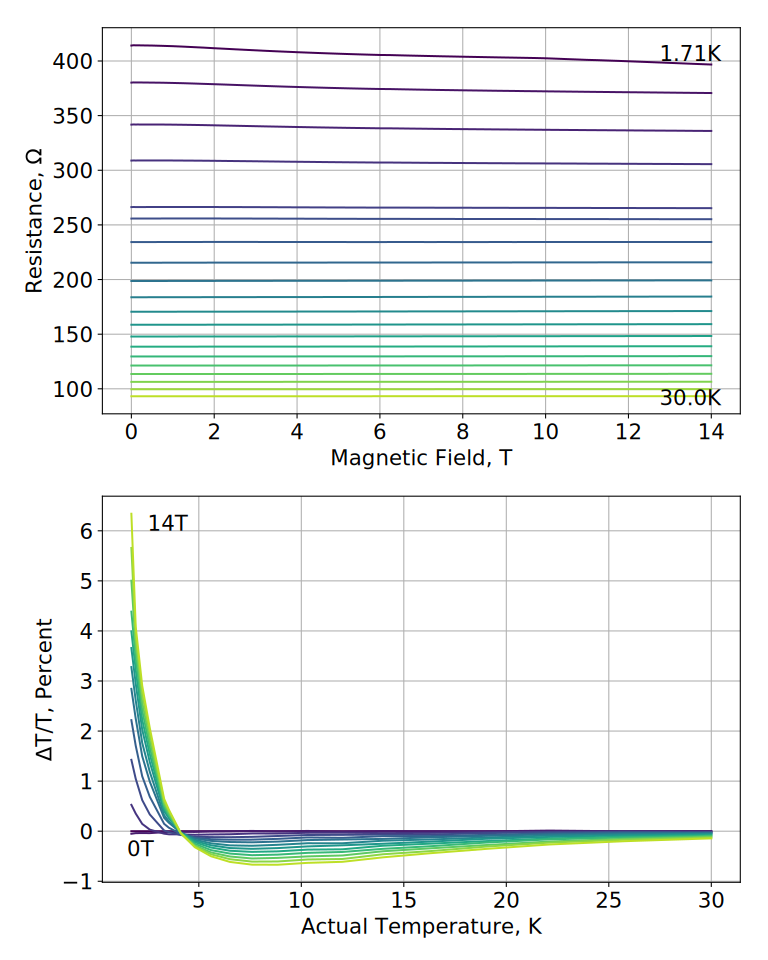
\includegraphics[width=\textwidth]{figures/cal_cernox_1.pdf}
\caption[Example Cernox Field Calibration]{Example Cernox Field Calibration. Top: Magnetoresistance of a
Cernox thermometer. Bottom: Field calibration curves for the same
thermometer.
\((T_{\mathrm{apparent}} - T_{\mathrm{actual}})/T_{\mathrm{actual}}\) is
plotted versus the actual temperature. \label{cernox_fieldcal}}
\end{figure}

Regardless, there is a great deal of scientific value in thermal
measurments performed in strong magnetic fields. Heat capacity provides
a generic method for identifying phase transitions, and thermal
transport is sensitive to excitations in a solid which do not carry
charge and thus can't be studied with electrical transport methods.
Thus, it is our goal to develop new methods for accurately and precisely
measuring temperature in the presence of intense magnetic fields. The
scientific potential of these methods and the experimental techniques
they make possible will be underscored in the next section. For more
information about thermometry and its application in experimental
condensed matter physics, chapter 5 of \cite{Ekin2006} is an invaluable
reference.

\section{Quantum Criticality in Strontium Titanate}
\begin{figure}
	\caption[Dielectric constant of Strontium Titanate]{Top: Dielectric constant of Strontium Titanate as a function
		of temperature, plotted as 1/$\epsilon$ vs $T^2$ to show the
		linear trend. Bottom: Low temperature plot of $1/\epsilon$,
		showing that $\epsilon$ reaches a maximum at $T = 3.29$K. This
		data was taken using the VTI probe in our Janis cryostat, but
		reproduces the results of ~\cite{Rowley2014}.}
		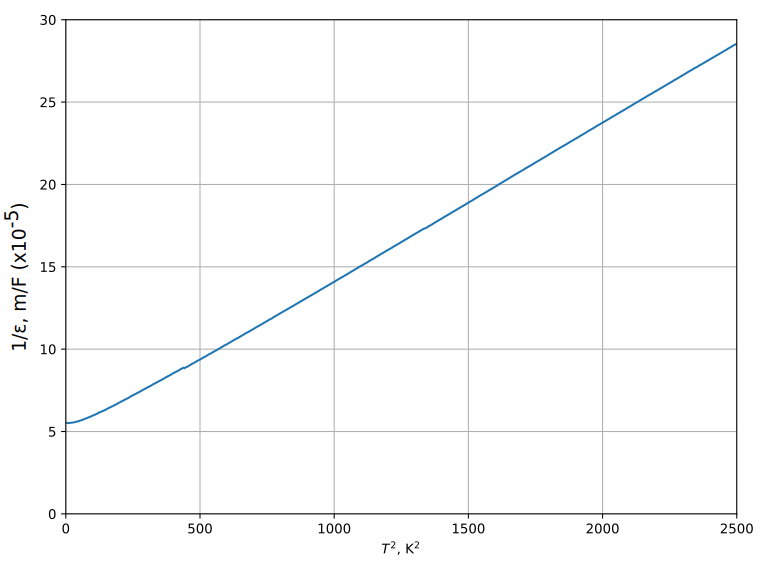
\includegraphics[width=0.9\columnwidth]{figures/STO_eps_vs_T.pdf}
		\includegraphics[width=0.9\columnwidth]{figures/STO_eps_vs_T_low.pdf}
		\label{sto_eps_vs_T} \end{figure}

\begin{figure}
	\caption[Sensitivity of STO test device]{Sensitivity of the Strontium Titanate device under test, plotted as the ``dimensionless'' quantity \(1/C dC/dT\).}
	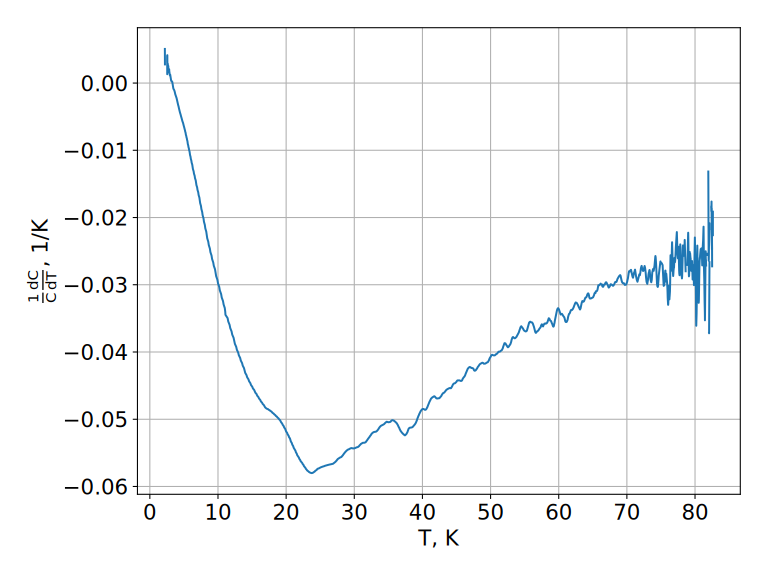
\includegraphics[width=\columnwidth]{figures/STO_dCdT_vs_T.pdf}
\end{figure}

\begin{figure} \caption[Dielectric constant of Potassium Tantalate]{Top: Dielectric constant of Potassium Tantalate
		(KTaO$_3$), another paraelectric material considered as a
		candidate for making capacitve thermometers. The linear trend
		when plotted as 1/$\epsilon$ vs $T^2$ is not as apparent as for
		SrTiO$_3$, and the overall change is not nearly as large.
		Bottom: Low temperature plot of $1/\epsilon$, as in figure
		\ref{sto_eps_vs_T}. The dielectric susceptiblity reaches a
		maximum at $T = 4.31$K, higher than that in SrTiO$_3$. As
		before, this data was taken using the VTI probe in our Janis
		cryostat, but reproduces the results of ~\cite{Rowley2014}.}
	
	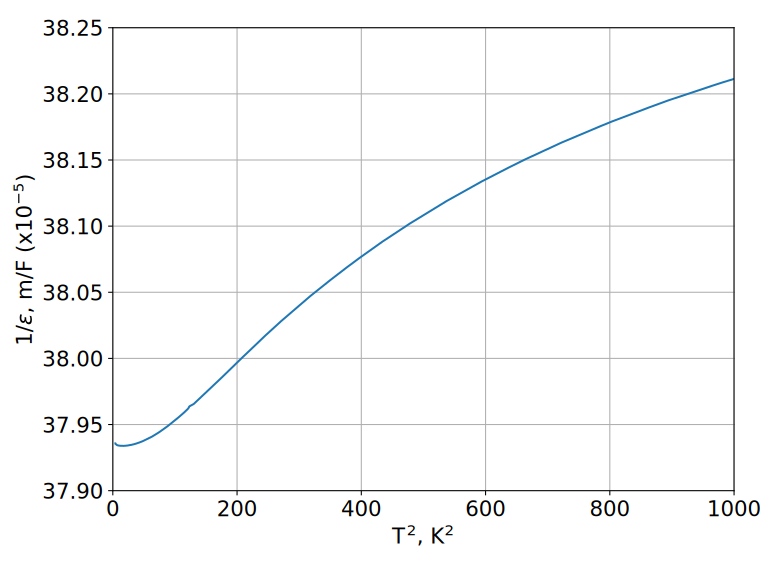
\includegraphics[width=0.85\columnwidth]{figures/KTO_eps_vs_T.pdf}
	\includegraphics[width=0.85\columnwidth]{figures/KTO_eps_vs_T_low.pdf}
\end{figure}

\section{Electronics For Measuring Capacitance}

\section{Strontium Titanate Thermometers}

Thermal transport measurements provide a versatile set of methods for probing
the physical properties of matter. Among thermal transport properties, the
thermal Hall effect shows promise for probing the ground state of many materials
of physical interest.  The thermal Hall effect, also known as the Righi-Leduc
effect,  is a thermal analogue of the standard Hall effect in which a thermal
gradient is applied across a sample in a magnetic field resulting a secondary
orthogonal thermal gradient. In this sense, a thermal Hall conductivity
$\kappa_{xy}$ is analogous to the Hall conductivity $\sigma_{xy}$.  While
$\sigma_{xy}$ in general contains information about the charged excitations
(electrons or holes) in a material, $\kappa_{xy}$ in principle contains
information about all the low-energy excitations. As a result the thermal Hall
effect has been of great theoretical interest for several years. In particular,
there has been some work that indicates that this technique may prove useful for
the study of strongly-correlated topological insulators (TIs) and
high-temperature superconductors. The thermal Hall effect is proposed to reveal
the experimental signature of different kinds of surface states\cite{Wang2014}:
free fermion TIs with a single Dirac cone, and two types of topological
paramagnet with spin-liquid behavior. Traditional Hall effect measurements can
distinguish some of these phases, but specific classification requires
measurement of the thermal Hall conductivity. Further theoretical studies
suggest that the thermal Hall effect could be used to study the quantum phase
transition from an Ising-like state with bosonic excitations to Majorana
fermions in the topological superconductors with supersymmetry~\cite{Grover2014}.

However, despite the intense theoretical interest in the thermal Hall effect,
the technique remains difficult to implement experimentally. A few interesting
measurements have been made in ferromagnets\cite{Onose2010}, frustrated quantum
magnets\cite{Hirschberger2015}, and cuprate superconductors\cite{Cvetkovic2015}, but
the experimental complications of accurately measuring temperature in an intense
magnetic field has prevented the technique from being applied more generally.
Because of the potential value of this technique for studying strongly
correlated materials and other materials of interest, we have sought to devise a
simple method for making these measurements. In particular, we wish to develop a
method which can be used on a wide variety of materials and throughout a large
temperature range, while being independent of the magnetic field.

In order to accomplish this, we have developed thermometers which measure
temperature by measuring the dielectric constant $\epsilon$ of strontium
titanate (SrTiO$_3$). High quality wafers of SrTiO$_3$ are generally available
for purchase, and the material is durable and relatively easy to work with. Its
value as a thermometer comes from the fact that its dielectric constant
increases by up to a few orders of magnitude at low temperature. This comes from
the fact that SrTiO$_3$ is very close to a quantum critical
point\cite{Rowley2014}. Materials similar to SrTiO$_3$, such as Barium Titanate
(BaTiO$_3$), undergo a ferroelectric transition at sufficiently low temperature.
On the other hand, SrTiO$_3$ is classical paraelectric at room temperature, but
is prevented from undergoing a ferroelectric transition due to long-range
interactions suppressing the ferroelectric state, causing it to remain a
(quantum) paraelectric instead. As a result, the dielectric constant does not
diverge a finite temperature, but instead saturates at about 4 K, depending on
the particular sample.

\begin{figure} \caption[A pair of STO thermometers]{A pair of STO thermometers, used to make thermal
  measurements. The background is a piece of graph paper with 1mm divisions, the
thermometers themselves are approximately 0.5 mm long, 0.5 mm wide, and 0.3 mm
thick.} \centering
\includegraphics[width=\columnwidth]{figures/thermometers_apl.jpg}\label{thermo_pic}
\end{figure}

\begin{figure} \caption[Example STO thermometer calibration]{An example calibration curve for an STO thermometer,
  showing both the capacitance (solid) and sensitivity (dashed) as a function of
temperature. The capacitance begins to saturate at low temperature, with the
sensitivity peaking around 25K. } \centering
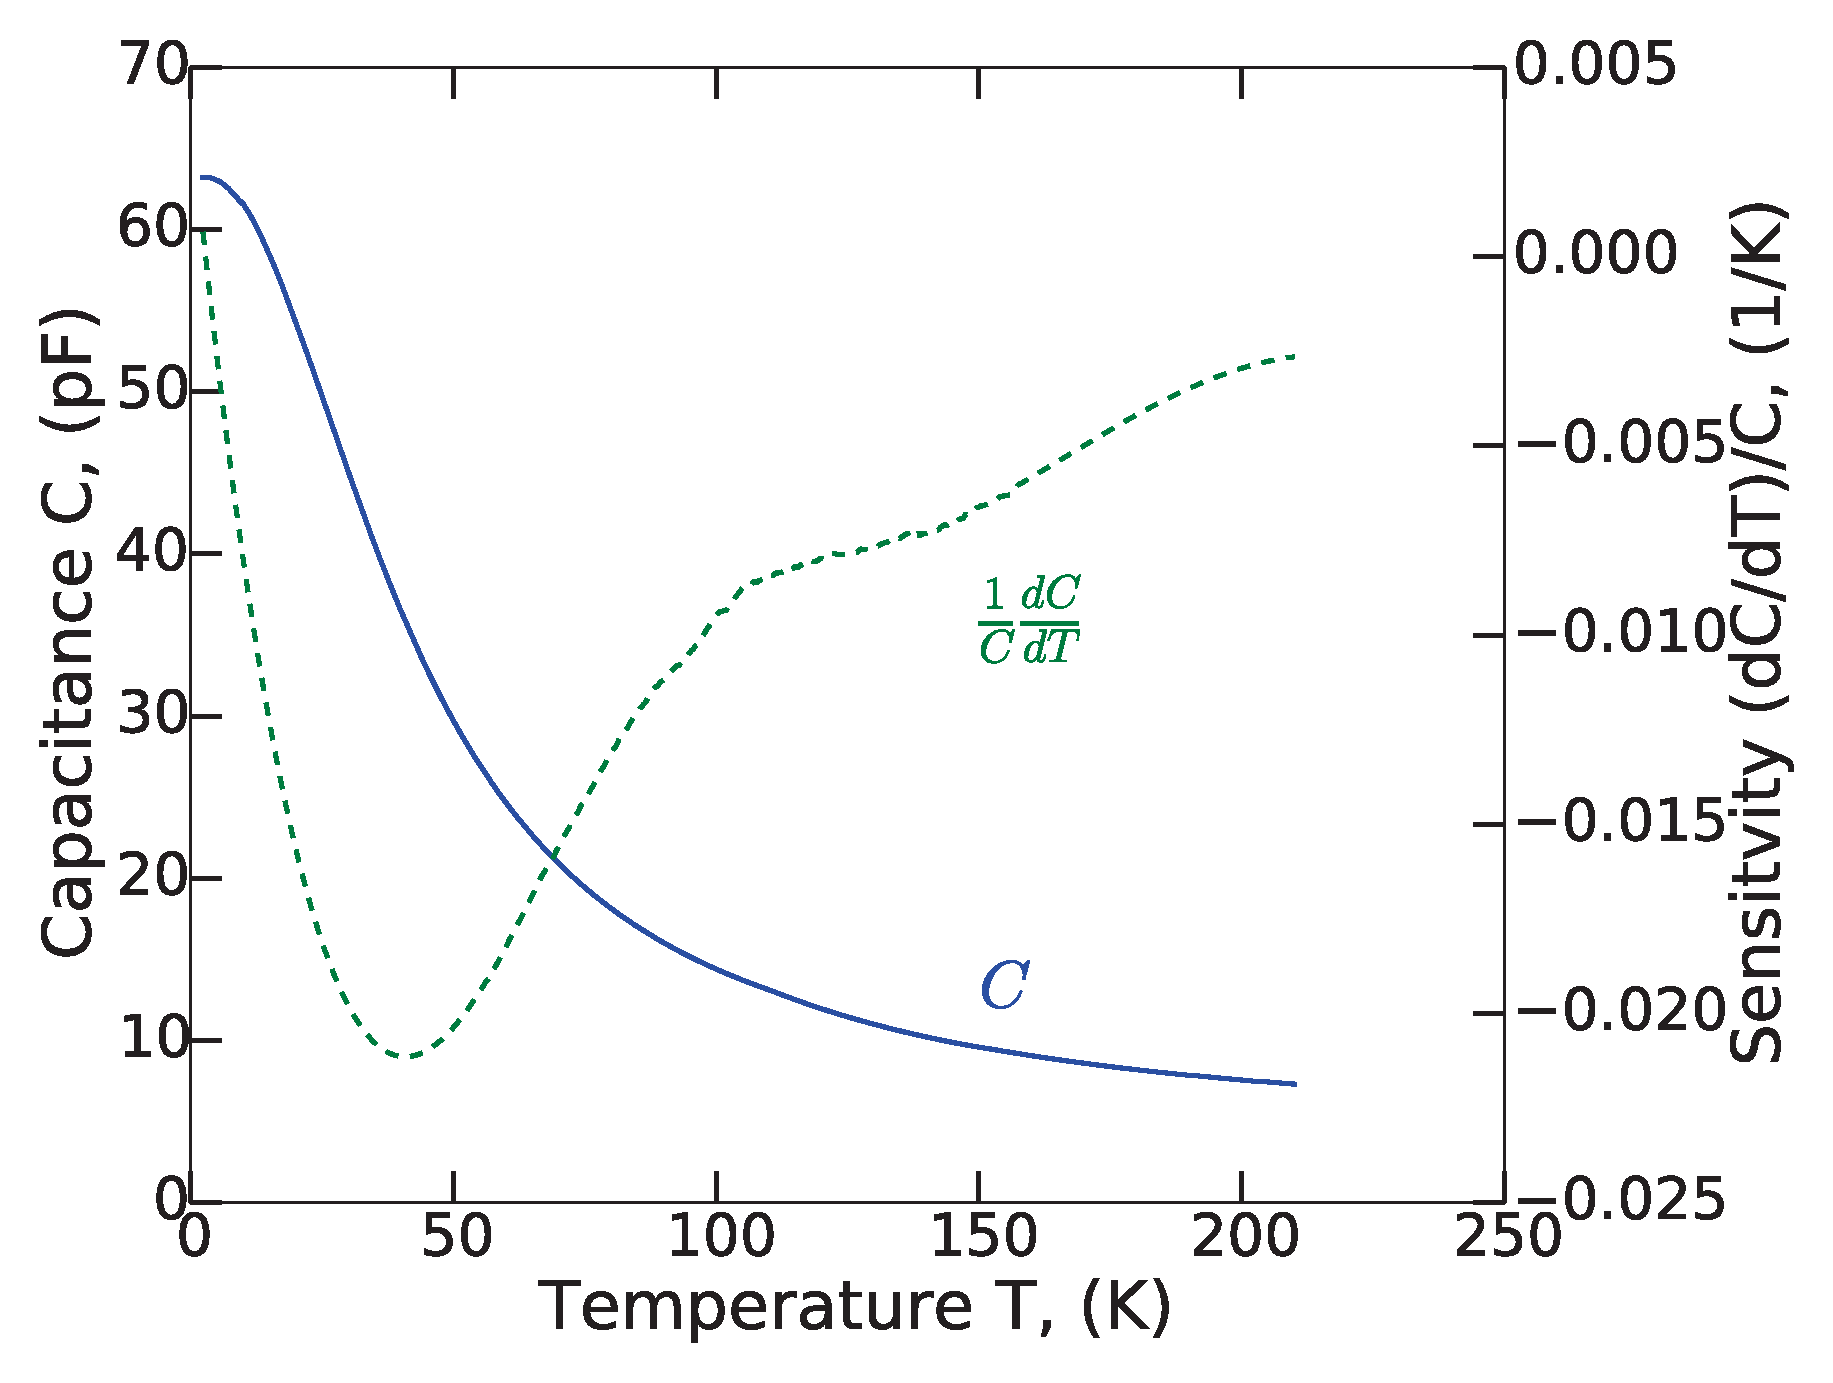
\includegraphics[width=\columnwidth]{figures/cvt_apl.eps}\label{cal_curve}
\end{figure}

In order to make a thermometer out of SrTiO$_3$, we take a small, thin (0.1 mm)
sample of the material (purchased from the MTI corporation)\cite{MTICorp} and
evaporate gold contacts on to either face.  These contacts form a parallel-plate
capacitor, and by measuring the change in the capacitance we measure the
dielectric constant and by proxy the temperature.  Figure~\ref{thermo_pic} shows
a pair of assembled thermometers.  The thermometers are approximately 0.5 mm
long, 0.5 mm wide, and 0.3mm thick, and the electrical leads are a pair of 25
$\mu$m diameter phosphor bronze wires.  Figure~\ref{cal_curve} shows an example
calibration curve for an SrTiO$_3$ thermometer. Both the capacitance and
sensitivity of the thermometer are shown from 4 K up to room temperature. The
magnitude of the sensitivity increases (note the sign, increasing dielectric
constant corresponds to decreasing temperature) up to about 25 K before
decreasing and reaching a maximum value below 4 K. The particulars depend
somewhat on the individual thermometer, notably, some do not reach a maximum
value at all above 1.5 K, the lowest temperature at which we calibrated the
thermometers used in this experiment. We believe this to be due to variance in
our process for making the thermometers, in particular the amount of heat they
are exposed to when the leads are attached and the resin surrounding the wafer
is cured. Because of this, they must be calibrated \textit{in situ} for each
experiment.  However, the general trend is the same, with the sensitivity being
greatest around 20 to 40 K. Using our capacitance bridges (an Andeen-Hagerling
2700A digital bridge and a General Radio 1615-A analog bridge), we can reliably
measure a change in capacitance of about 1$\times$10$^{-5}$ pF. This corresponds
to change in temperature of 0.1 mK. Other measurements~\cite{Hirschberger2015}
using resistive thermometers quote a resolution of 0.2 - 0.4 mK. This is after
extensive field calibration of the thermometers, a time-consuming process which
these thermometers eliminate.

\begin{figure} \caption[Field response of an STO thermometer]{A test of the response of an STO thermometer to an
    applied magnetic field, taken at 4.2K.  The field starts at zero, scans to
    10T (blue), then to -10T (green), and then back to zero (red).  The relative
    change in the capacitance $(C - C_0)/C_0$ remains less than
  3$\times$10$^{-4}$, corresponding to change of about 20 femtofarads. This
change in capacitance is possibly due to the shifting of the leads to the
capacitor plates due to the field, rather than anything intrinsic to STO.}
\centering 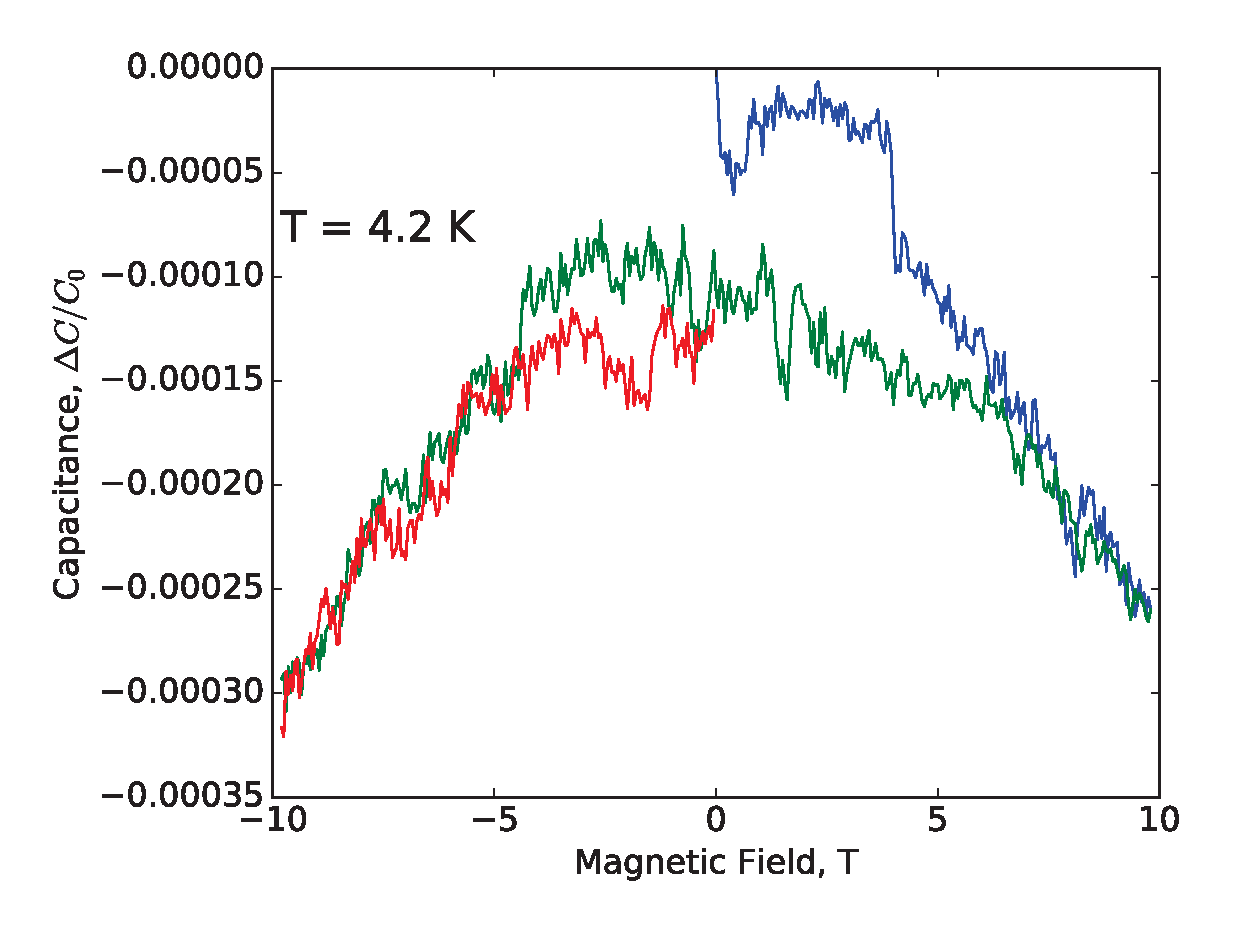
\includegraphics[width=\columnwidth]{figures/cvb_apl.eps}\label{b_test}
\end{figure}

Of course, in order to perform well for making thermal Hall effect measurements,
these thermometers must not be sensitive to an applied magnetic field.
Figure~\ref{b_test} shows the relative change in capacitance $(C-C_0)/C_0$ of a
sample thermometer measured under a magnetic field from -10 T to 10 T.  The
magnitude of the change in capacitance remains less than 3$\times$10$^{-4}$, a
few parts in ten thousand, below 10 T at 2 K. Compare this to resistive
thermometers, which may have magnetoresistance of a few percent or greater in
this temperature range\cite{Heine1998,Goodrich1998}. We are not sure what the nature
of this small field dependence is, as the dielectric constant should be
independent of applied magnetic field. However, at least some of the change may
be related to the slight shifting of the thermometer leads as the field is
swept.

Another issue concerning the suitability of these thermometers for measuring the
thermal Hall effect, particularly relevant at low temperature, is the heating
caused by the thermometers themselves. As the temperature decreases and the
dielectric constant increases, the dissipative losses from the capacitor
increase as well. These increase to about 60 nW at low temperature. For our
current experiment, which applies 1 mW of power across the sample, this is not a
concern. In general, however, this is not insignificant. 60 nW corresponds to an
excitation of 1 V. Decreasing the excitation will quadratically decrease the
heating power, however this comes at the cost of the sensitivity of the device.
This at least gives us some room to adjust the parameters to fit the particular
experiment. As our process for assembling the thermometers improves, we should
be able to mitigate this source of heat by reducing resistive loss across the
capacitor.  Despite the difficulty with the thermometer heating, the fact that
the thermometers are insensitive to magnetic field at low temperature makes them
good candidates for making a variety of thermal measurements.

Furthermore, the heat loss through the thermometer leads are negligible compared
with the sample's thermal conductance. Each thermometer has a pair of 25 $\mu$m
diameter phosphor bronze leads, with a thermal conductivity of 69.9 $\mathrm{W/m
  \cdot K}$ at room temperature given by the manufacturer (California Fine Wire
  Co)~\cite{CFW}. On the other hand, bismuth has a thermal conductivity of 7.87
  $\mathrm{W/m\cdot K}$ at room temperature~\cite{Ekin2006}.  Given the dimensions
  of our sample and the fact that there are two thermometers with four leads
  total, this results in a thermal conductance of 1.6 $\mathrm{mW/K}$ through
  the sample compared to 0.027 $\mathrm{mW/K}$ through the leads, almost 60
  times smaller. Since the thermal conductivity of bismuth goes up below room
  temperature~\cite{White1958}, while that of phosphor bronze goes
  down~\cite{Ekin2006}, the quality will only improve at the measurement
  temperatures.

  \begin{figure} \caption[Transverse temperature gradient of a bismuth crystal]{(Panel a): Transverse temperature difference as a
    function of applied magnetic field from -10 T to 10 T, taken at 130 K and
    measured using a pair of STO thermometers. The signal is composed of an
    symmetric part and an antisymmetric part.  (Panel b): Antisymmetric (solid)
  and symmetric (dashed) parts of the transverse temperature difference. The
antisymmetric part is the thermal Hall signal. Notice the difference in scales
for the two curves.} \centering\label{t_grad}
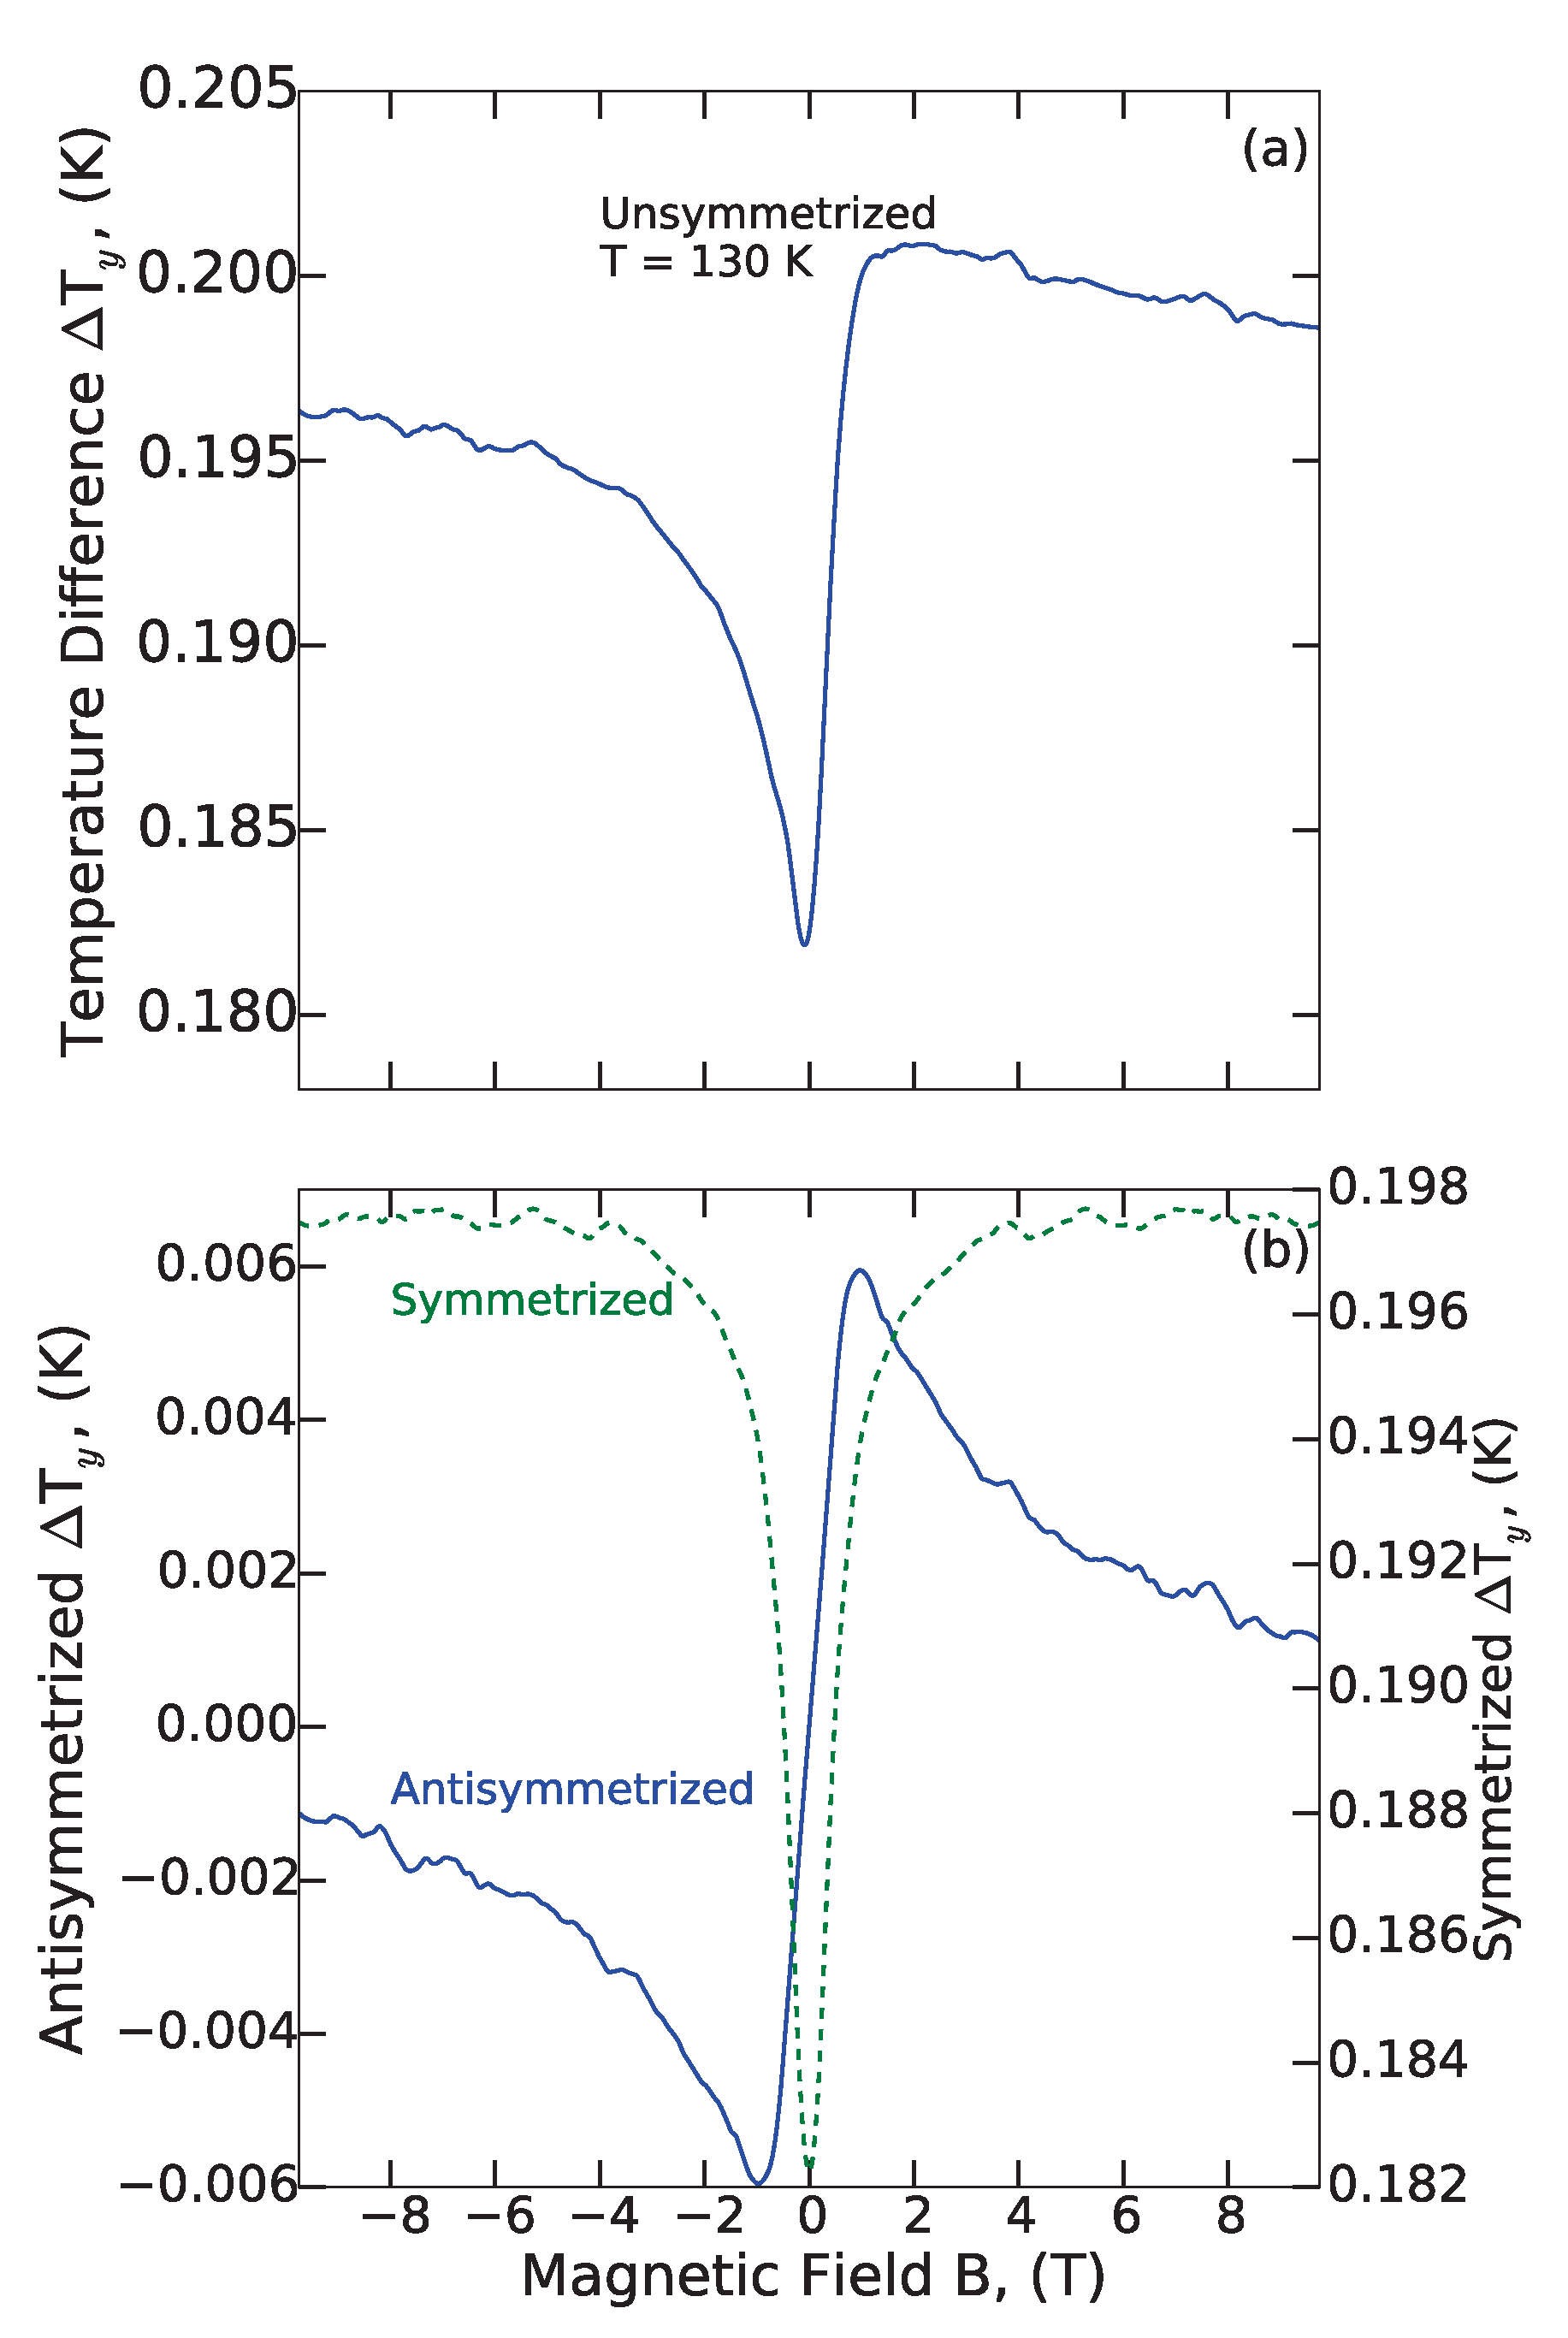
\includegraphics[width=0.9\columnwidth]{figures/rawCurve_apl.eps} \end{figure}

\section{Measuring the Thermal Hall Effect in Bismuth}

As a test of these thermometers' suitability for thermal Hall measurements, we
have measured the thermal Hall coefficient of Bismuth metal. Bismuth is one of
the most studied condensed matter systems, being the material in which a host of
physical phenomena were first discovered. Examples include quantum oscillations
and the de Haas van Alphen effect\cite{deHaas1930}, and perhaps more directly
related to the field of thermal transport measurements, the Seebeck
effect\cite{Seebeck1922}. It has a unique electronic structure, being a semimetal
with Dirac-like dispersion\cite{Lui1995, Li2008}, strong spin-orbit
coupling\cite{Yafet1963}, and pronounced diamagnetism\cite{Shoenberg1936}. More
recently, it has been studied\cite{Emoto2016} for its ability to convert spin
current to charge current along with the ferromagnetic insulator
yttrium-iron-garnet through the inverse spin Hall effect and inverse
Rashba-Edelstein effect. This interplay of electronic, magnetic and thermal
phenomena make bismuth a promising candidate for observing the thermal Hall
effect using our capacitive thermometry technique.

The thermal Hall effect on crystalline bismuth has been carried out by W.
Kobayashi \textit{et al.}\cite{Kobayashi2012} down to 75 K and magnetic fields up
to $\pm$3 T. Using our thermometers, we sought to extend this measurement to
lower temperatures and higher fields. A resistive heater was mounted on a single
crystal of bismuth metal, in order to generate a temperature gradient. A pair of
SrTiO$_3$ thermometers were mounted in order to measure the transverse
temperature gradient. The thermometers were glued to the surface of the sample
and then coated in Type 120 silicone thermal joint compound to ensure good
thermal contact with the sample. An example set of temperature gradient data is
shown in Figure~\ref{t_grad}. Two pairs of thermocouples were mounted as well,
one longitudinal and one transverse, in order to independently measure the
temperature gradients \textit{in situ}. An additional resistive thermometer was
mounted nearby to calibrate the SrTiO$_3$ thermometers in zero field.  The
heater was repeatedly turned on and off, and the gradients in each direction
measured. Simultaneously, the applied magnetic field was swept between -10 T and
10 T. This allowed us to measure the field dependence of the thermal Hall
coefficient.

\begin{figure} \caption[Thermal Hall conductivity of bismuth]{Thermal Hall conductivity, computed from the
    transverse temperature difference measured using the STO thermometers from
    -10 T to 10 T. Curves for a few temperatures between 90K and 175K (Panel a)
    and between 40K and 80K (Panel 6). The signal appears to get smaller at
lower temperature, disappearing at 60K.} \centering\label{kappaxy}
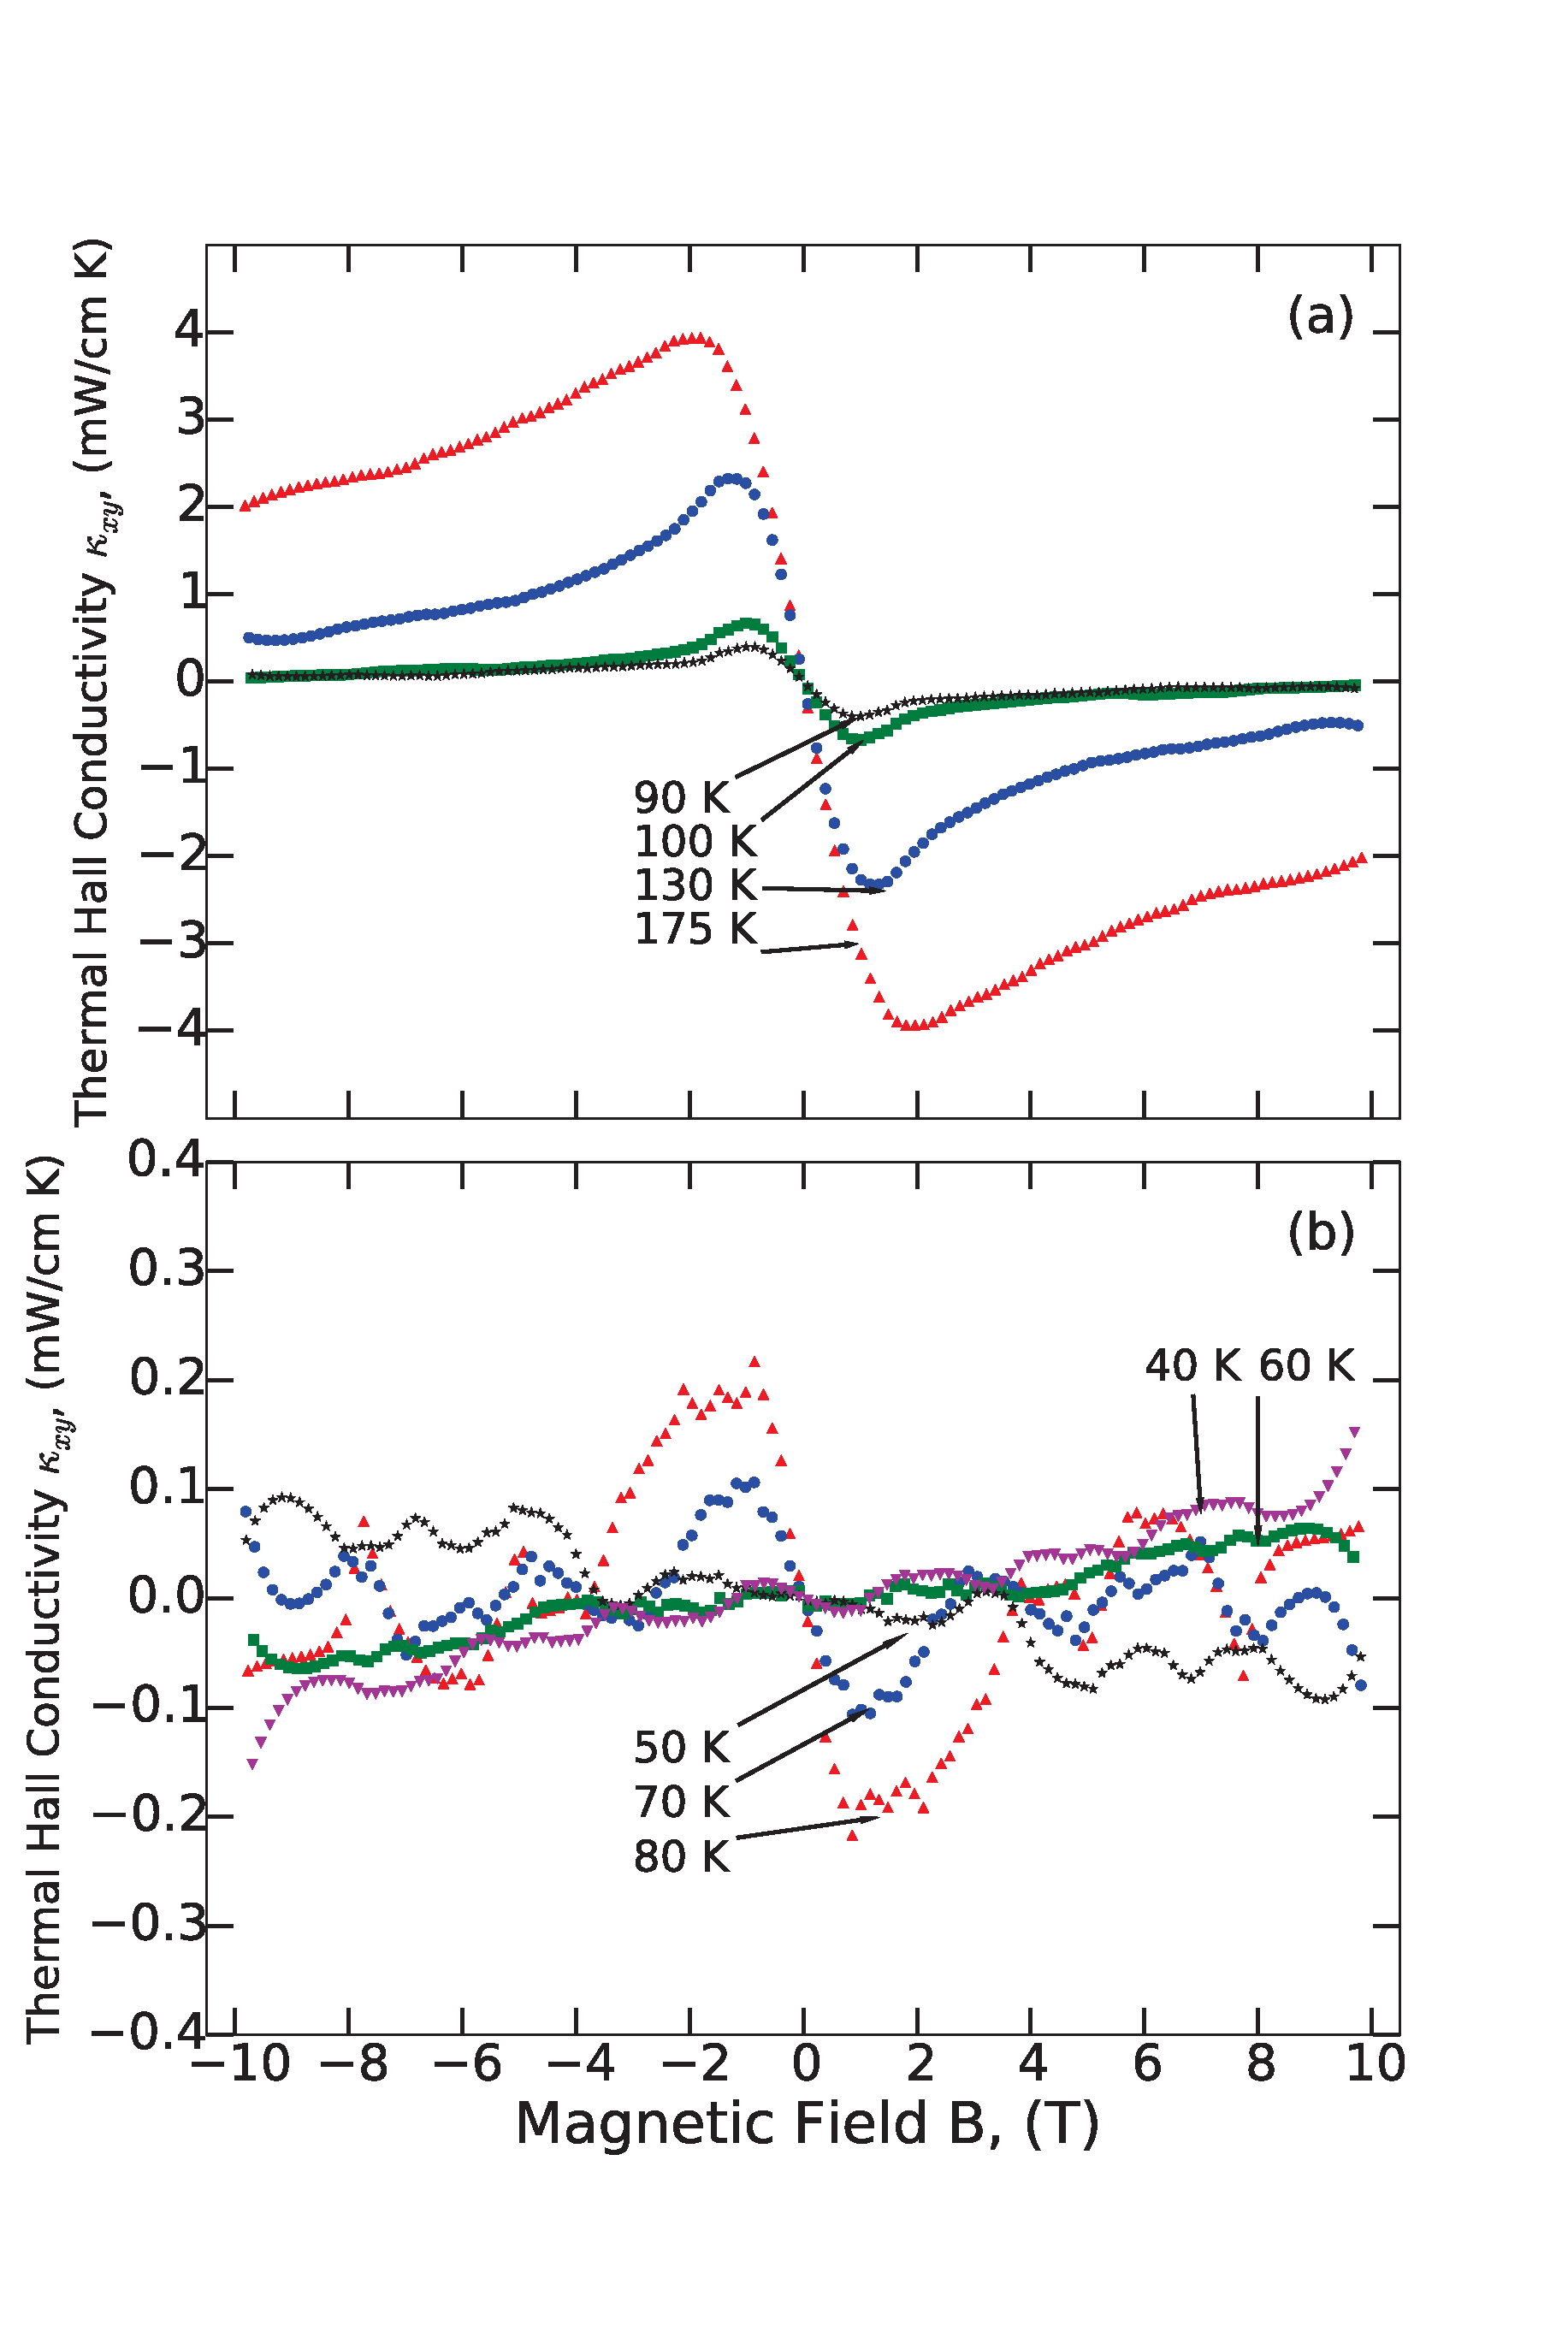
\includegraphics[width=\columnwidth]{figures/kappaxy_apl.eps} \end{figure}

Similar to what was measured before\cite{Kobayashi2012}, the thermal Hall
conductivity is strongly nonlinear, reaching a maximum below 2 Tesla and
decaying down to zero at high field, as shown in Figure~\ref{kappaxy}.  It is
also largest at high temperature, becoming imperceptible below 50 K, where our
thermometers are most sensitive.  As a result, we are confident that this is not
an artifact of the capacitive thermometers. Thus we can see that the STO
thermometers are able to make sensitive measurements, detecting changes in
temperature below 1 mK in magnetic fields up to 10 T. Additionally, the fact
that they are relatively simple to produce makes them applicable to a wide
variety of measurements and samples. One remaining challenge is our ability to
push these measurements to lower temperature, suitable for use at helium-3 or
dilution refrigerator temperatures, where traditional methods of thermometry are
even more fraught\cite{Heine1998, Goodrich1998}. One promising line of study
involved isotopically substituting $^{18}$O into the strontium titanate wafers,
which has been shown\cite{Rowley2014} to drive them closer to the ferroelectric
quantum phase transition and thus continue the divergence of their dielectric
constant to lower and lower temperature. In any event, as this measurement has
shown, this method of thermometry holds great promise for enabling the thermal
properties of materials in intense magnetic fields.

In conclusion, miniature capacitive thermometers based on the paraelectric
material SrTiO$_3$ have been applied to measure the thermal Hall effect in
crystalline bismuth. A strong nonlinear thermal Hall effect is observed in the
intermediate temperature range. The miniature SrTiO$_3$ thermometers show very
little magnetic field dependence -- less than a factor of 3$\times$10$^{-4}$ up
to magnetic field 10 T. They are also quite sensitive, resolving the temperature
difference as little as 0.1 mK.

\section{Annealing Strontium Titanate in Oxygen-18}

\begin{figure} \caption[Strontium Titanate Annealing System]{Schematic of the annealing system used to produce oxygen-18 enriched strontium titanate wafers. The circles labled ``P'' are pressure gauges, and the circles with crosses are valves. Oxygen-18 is supplied from a gas cylinder, and can be stored in the cold trap for reuse.}
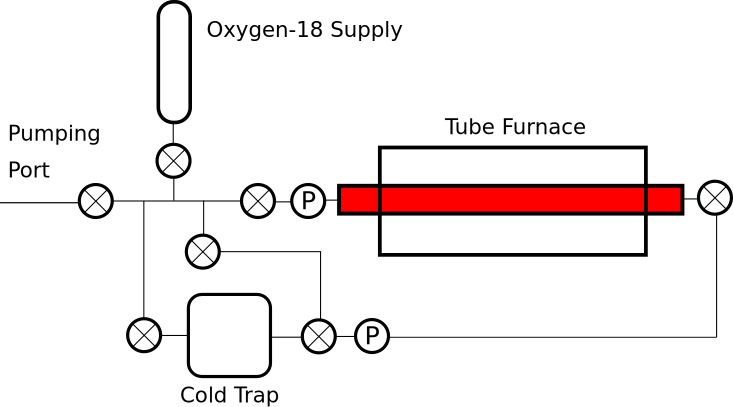
\includegraphics[width=\columnwidth]{figures/annealing_system.pdf}
\end{figure}

\begin{figure} \caption[Annealed STO thermometer reproducability tests]{Top: Reproducability tests for several annealed STO
	capacitor devices, measured in a liquid helium dewar using a dipstick
probe. The Oxygen-18 enrichment percentage is listed in table <TODO>. Note the
offset between the cool down and warm up traces for each device. Bottom:
Sensitivities for the same four devices. Although the capacitance varies
between devices and cool down/warm up, the sensitivity is roughly the same for
each.} 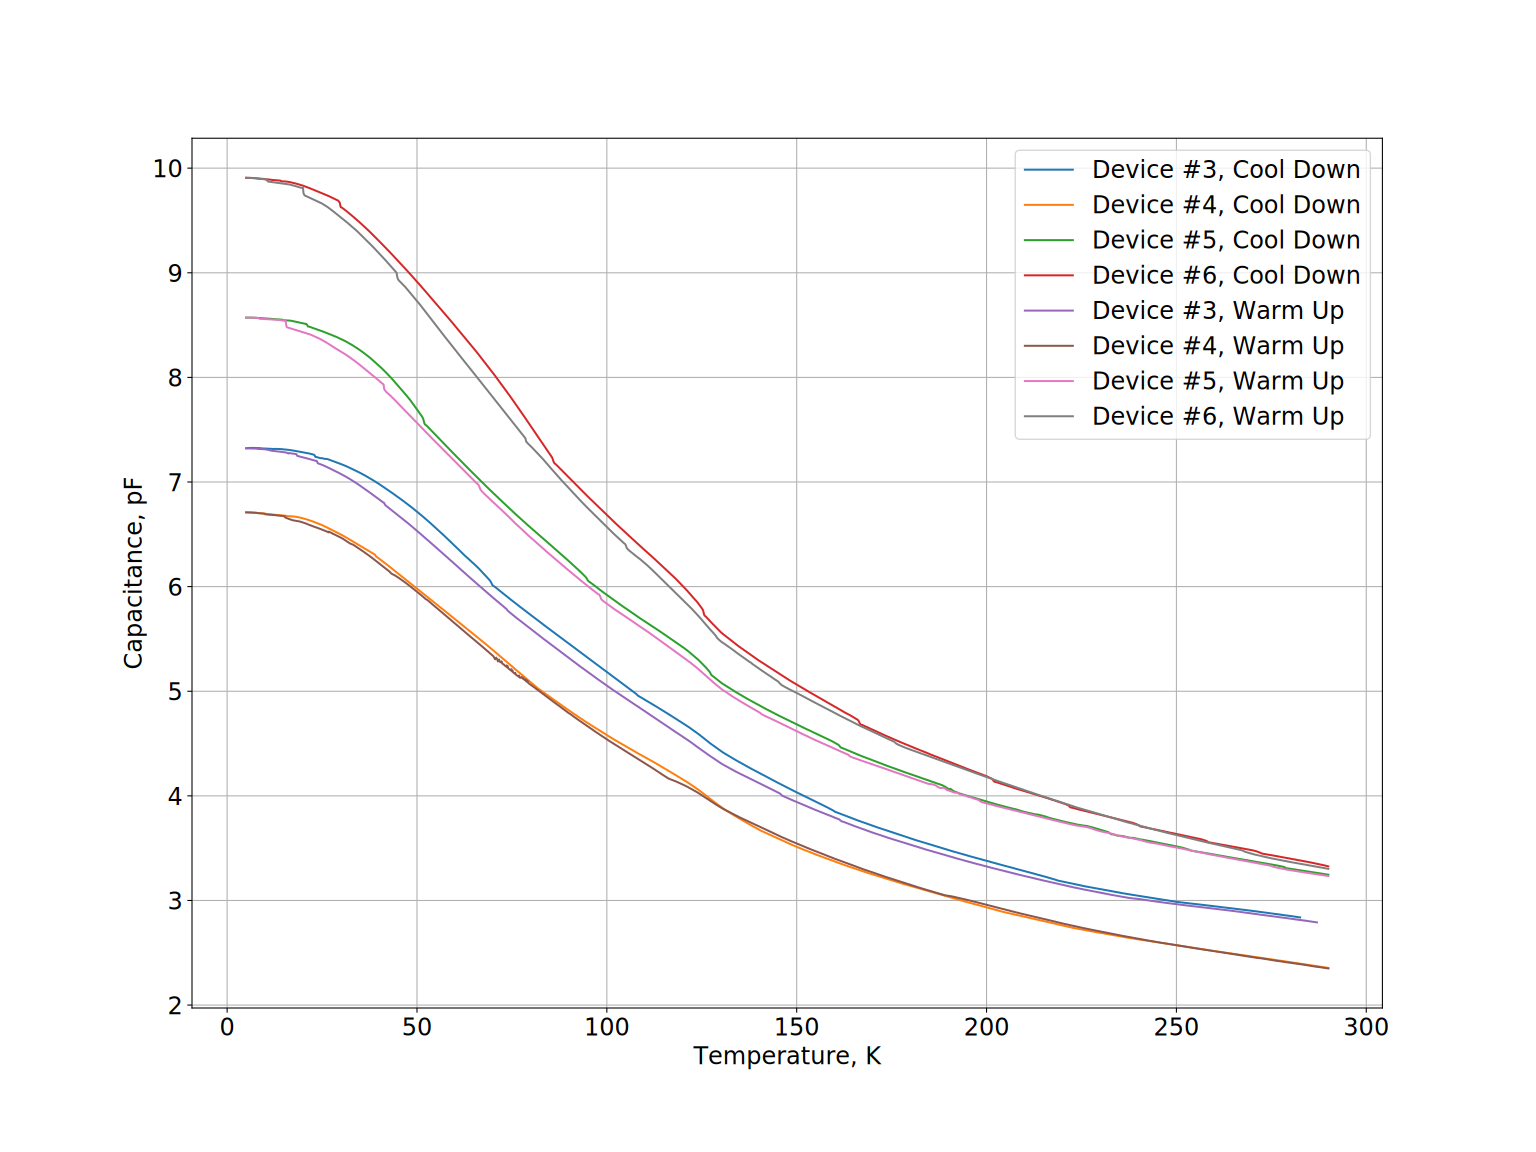
\includegraphics[width=0.9\columnwidth]{figures/annealed_sto_c_vs_t.pdf}
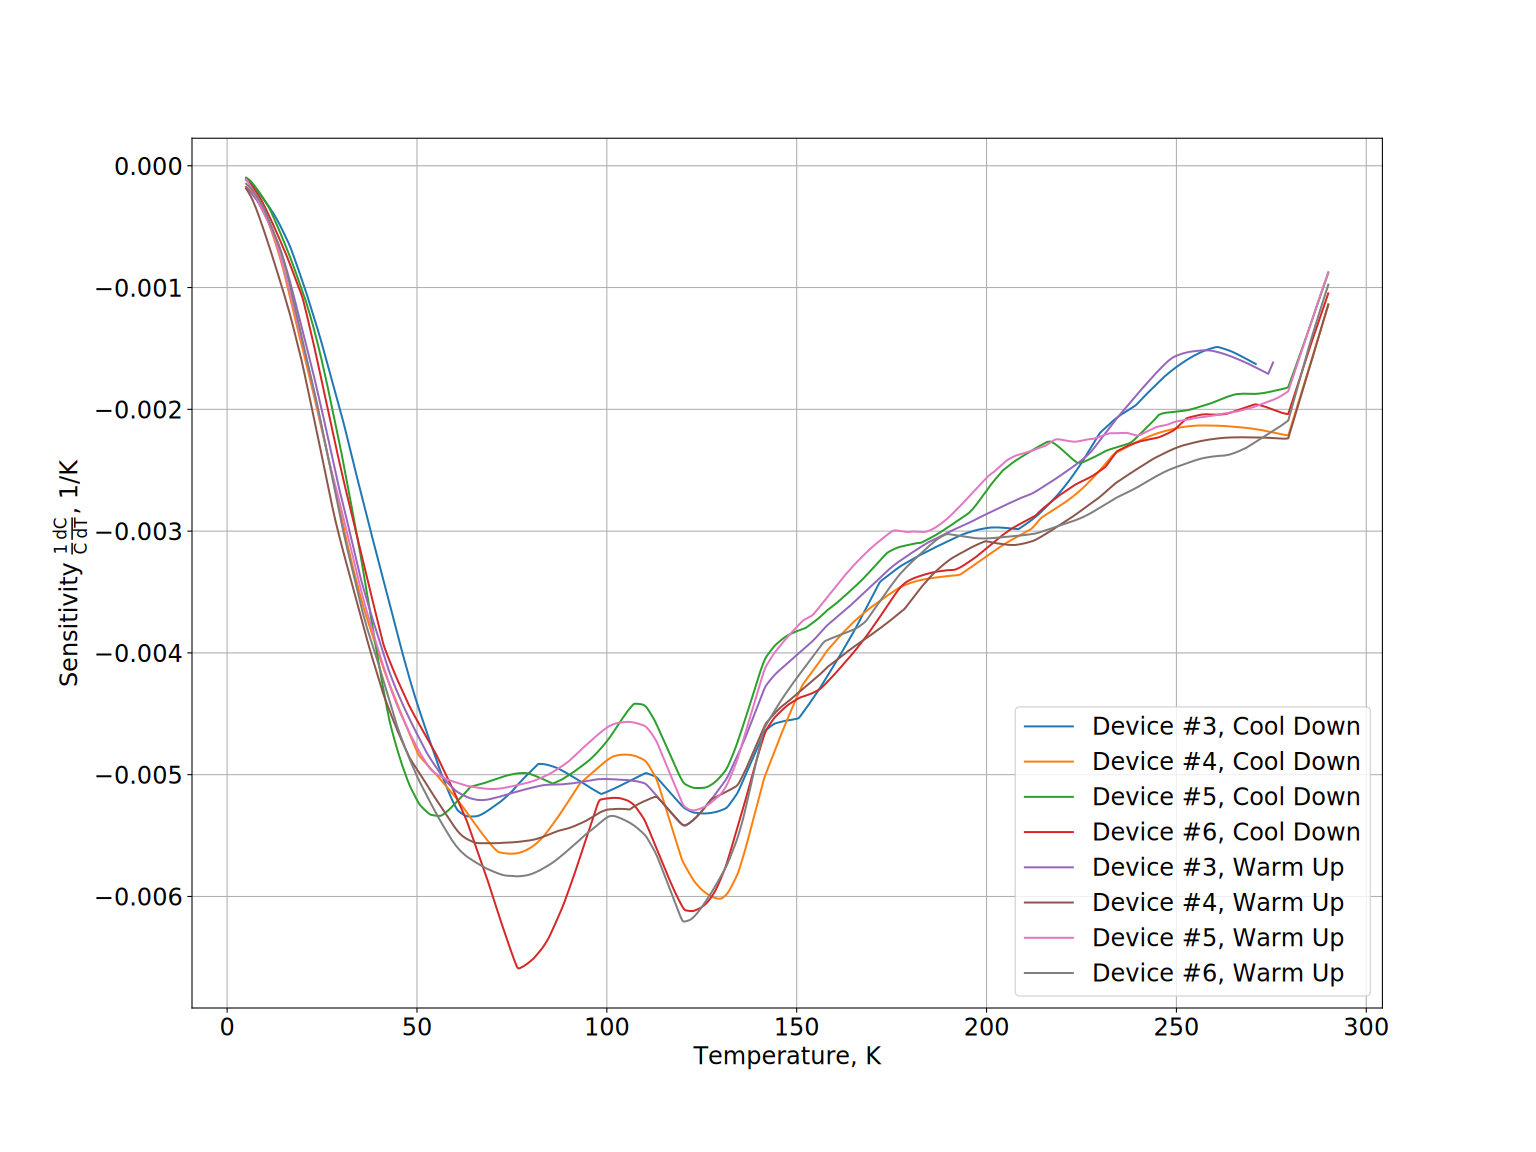
\includegraphics[width=0.9\columnwidth]{figures/annealed_sto_sens_vs_t.pdf}
\end{figure}

\begin{figure} \caption[Annealed STO thermometer dissipation]{Top: Dissipation for the annealed STO devices. Unlike
	the unannealed devices, the dissipation does not increase at low
temperature. Bottom: Heat capacity measurement of a strontium titanate wafer
(blue dots), measured using the Quantum Design PPMS. The measurement does not
show any power law behavior indicative of a phase transition, and so it has not
been doped into the ferroelectric regime. The cubic fit (orange line) is
indicative of simple insulating behavior.}
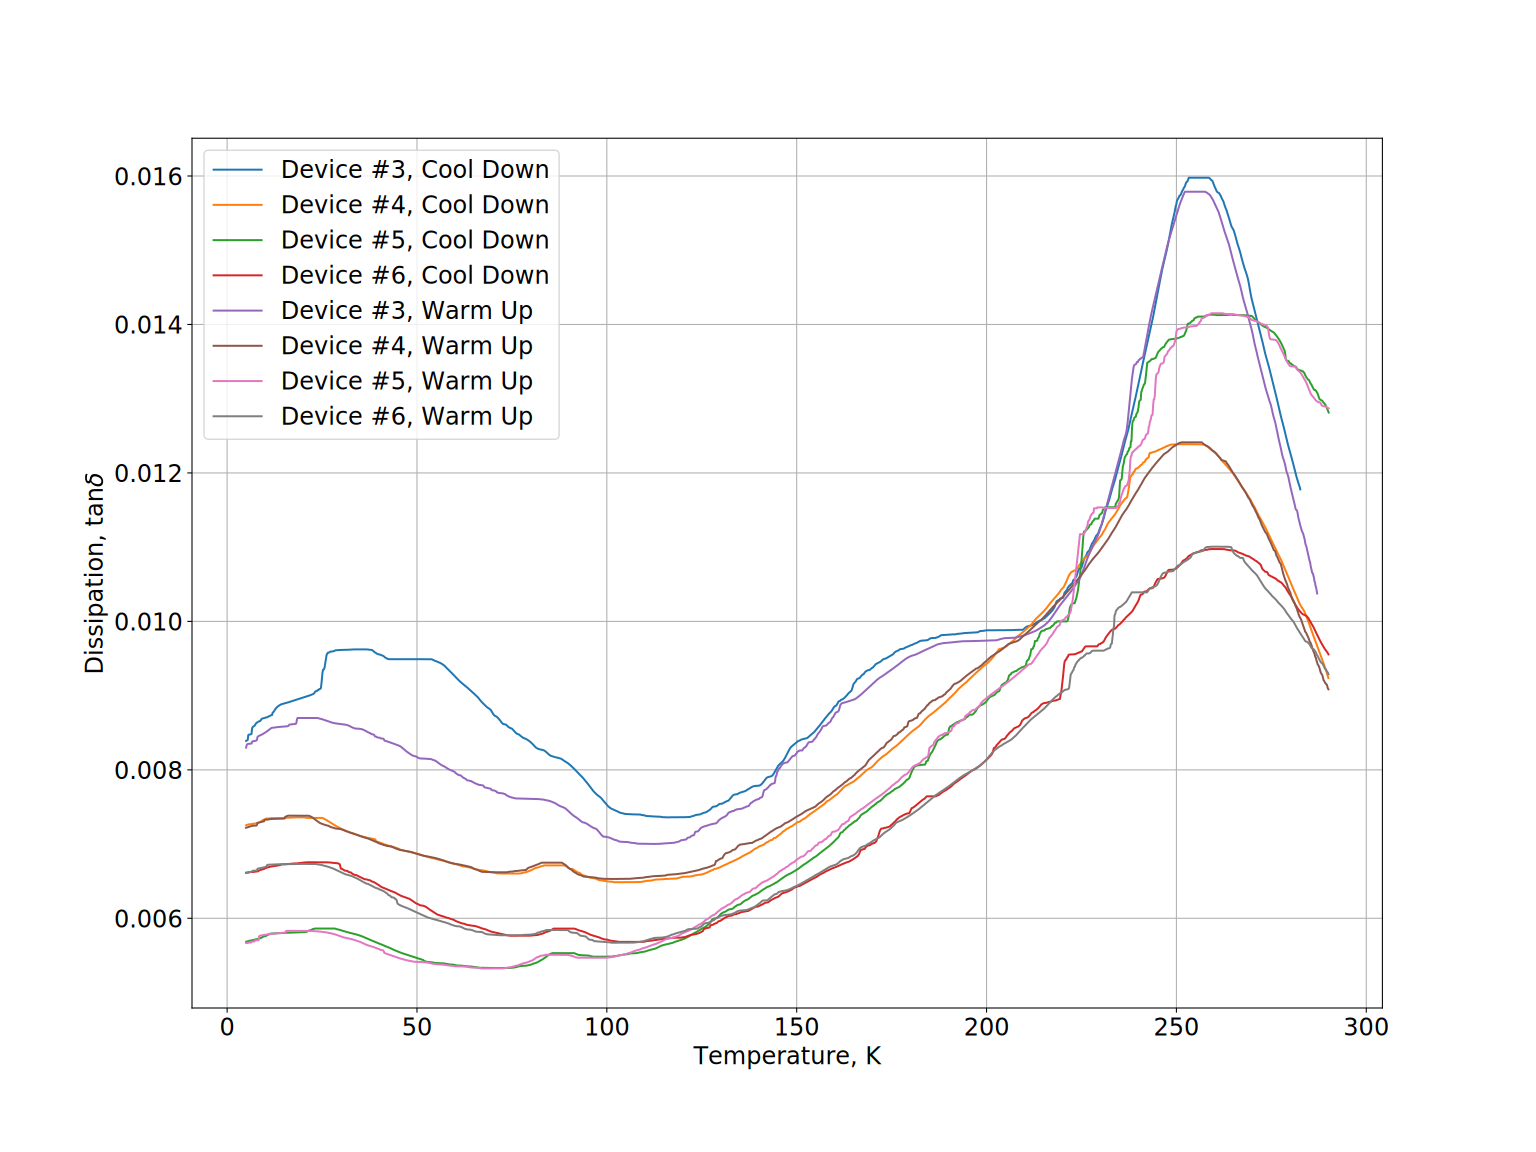
\includegraphics[width=0.9\columnwidth]{figures/annealed_sto_diss_vs_t.pdf}
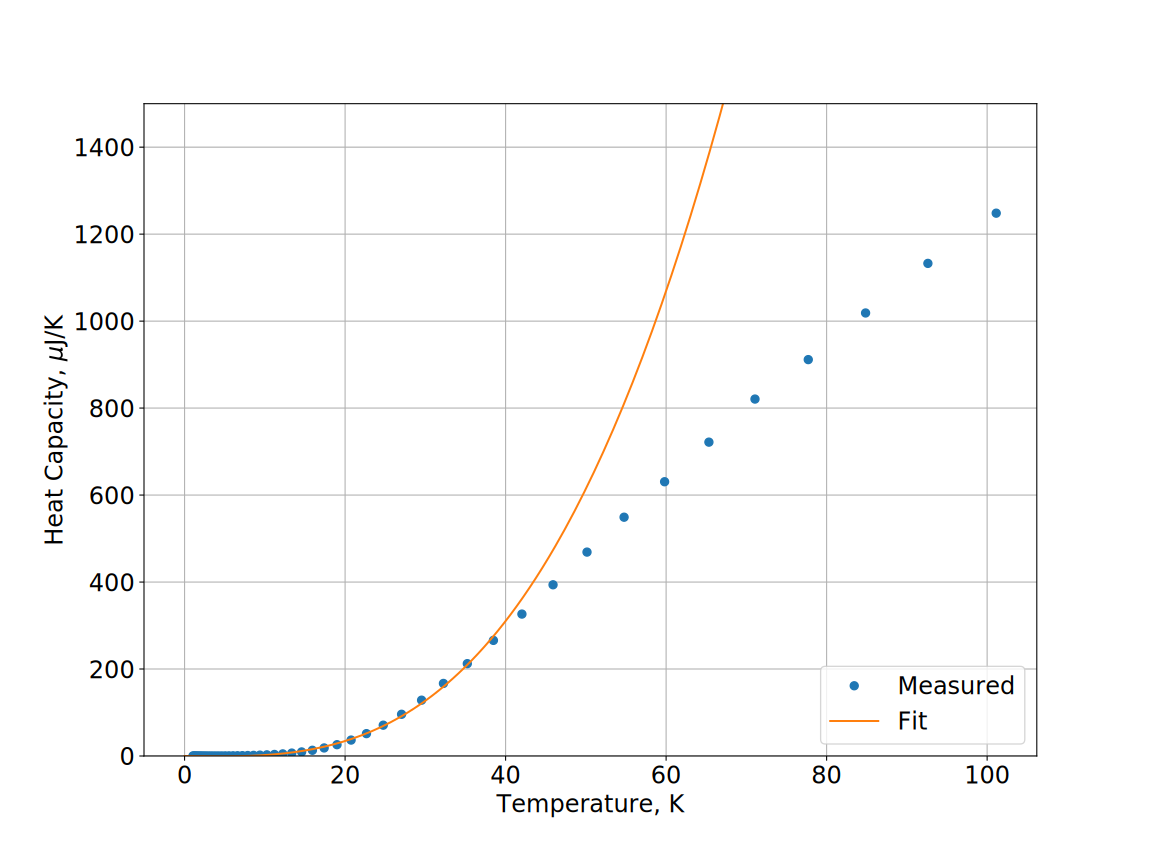
\includegraphics[width=0.9\columnwidth]{figures/annealed_sto_heatcap_vs_t.pdf}
\end{figure}

\begin{figure} \caption[Field response of an annealed STO thermometer]{Relative change in capacitance of an annealed STO
	thermometer in an applied magnetic field, measured up to 14 tesla in
the Quantum Design PPMS. The improved sample mounting in the PPMS eliminates
the background from the flexing of the wires.}
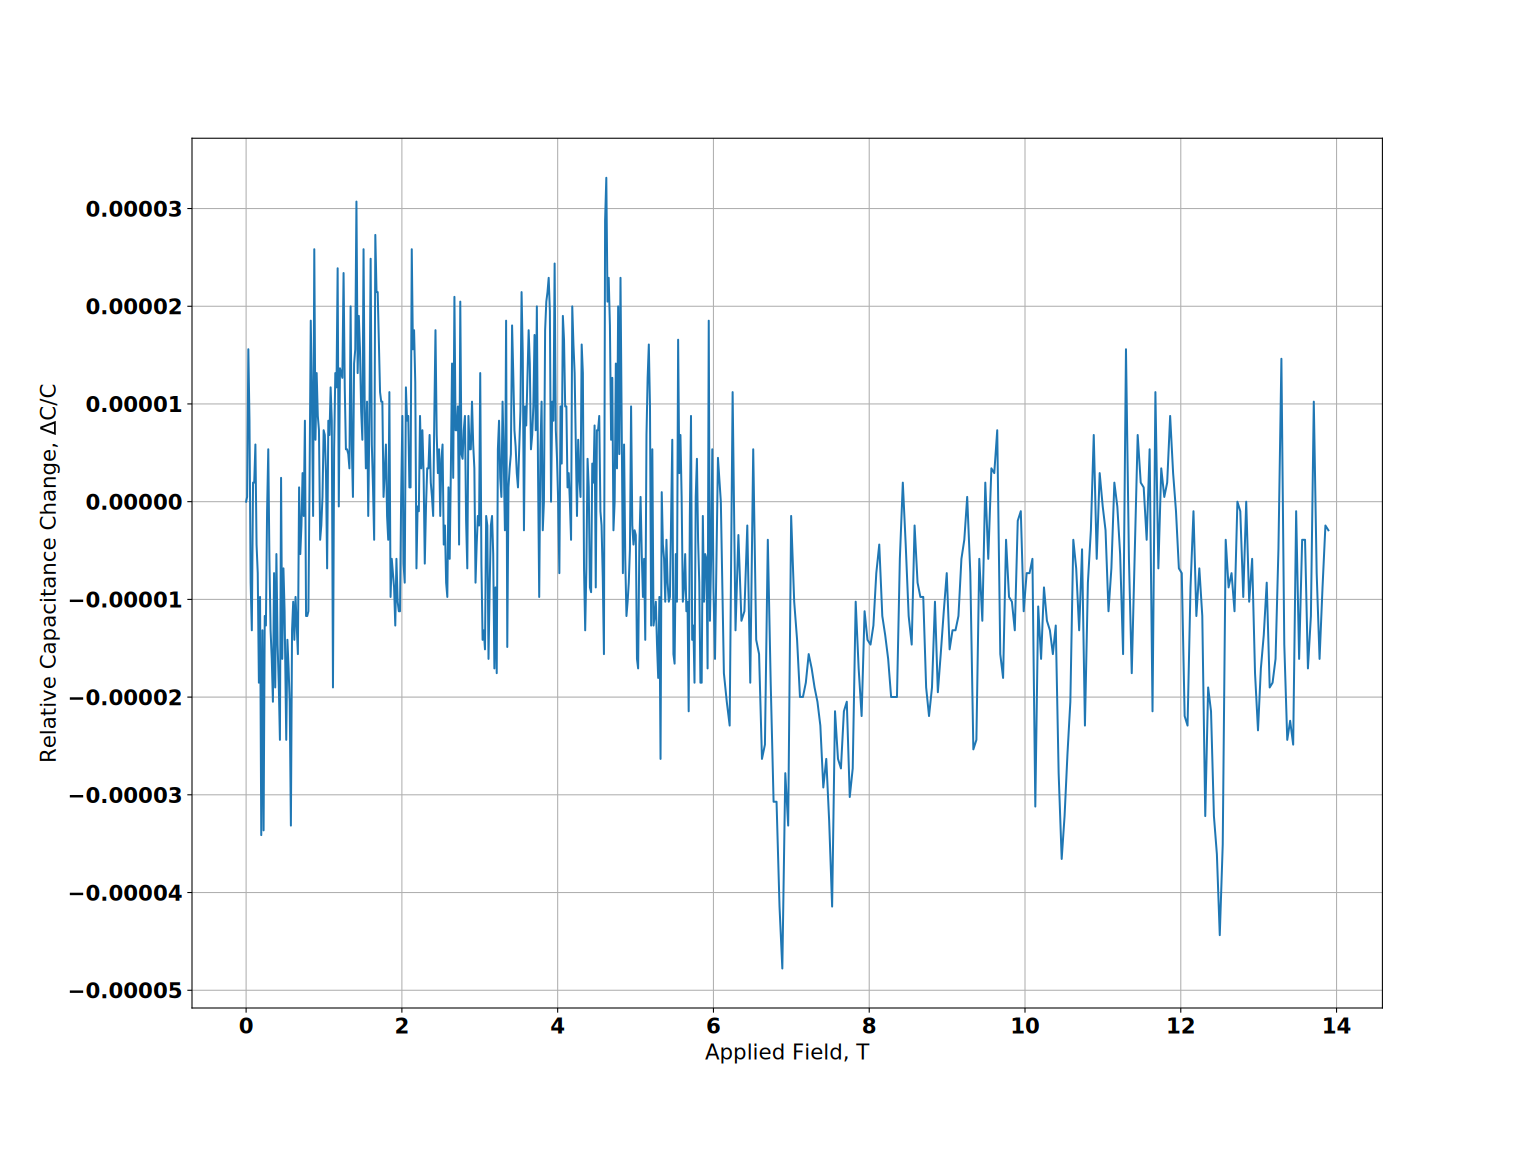
\includegraphics[width=\columnwidth]{figures/annealed_sto_dc_vs_b.pdf}
\end{figure}
	
\chapter{Thermal Measurements of Strontium Copper Borate}

\section{The Shastry-Sutherland Model}
\begin{figure}
	\caption[The Shastry-Sutherland lattice]{Schematic of the Shastry-Sutherland lattice. Each red circle has spin 1/2. The nearest-neighbor coupling $J$ is represented by the solid lines, and the intra-dimer coupling $J'$ is represented by the dashed line. Each spin is in exactly one dimer.}
	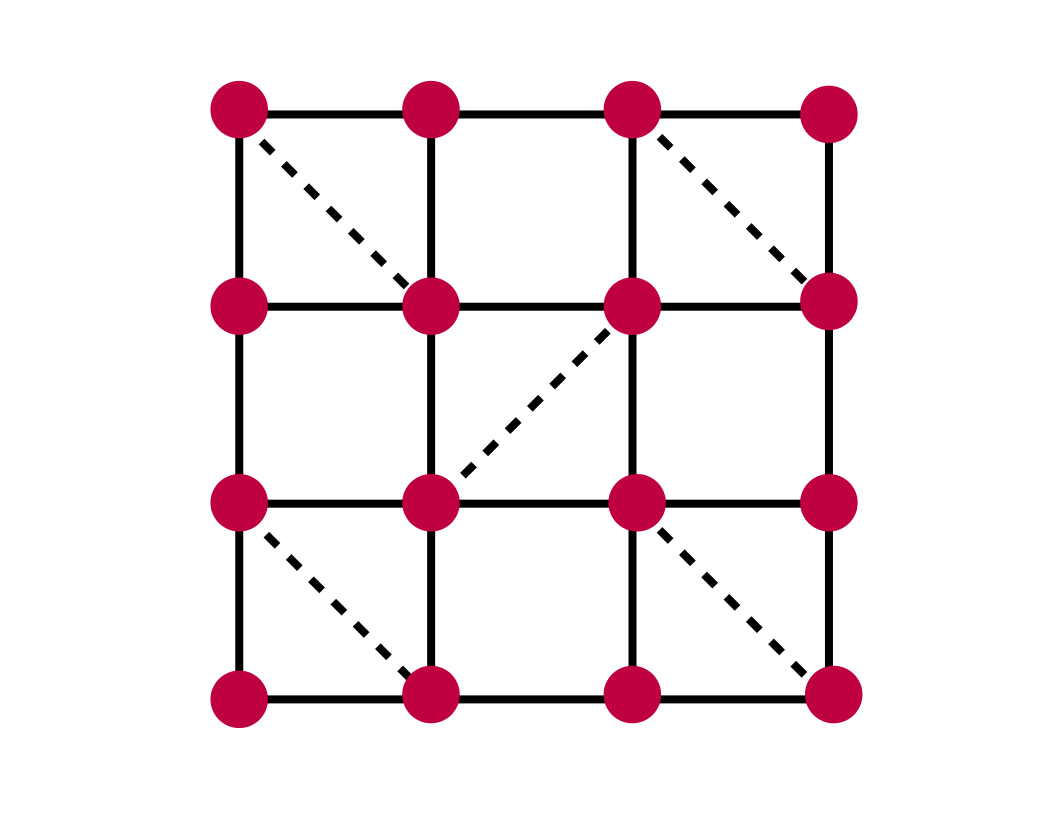
\includegraphics[width=\columnwidth]{figures/ss-model.pdf}
\end{figure}

\begin{figure}
	\caption[Crystal structure of strontium copper borate]{Crystal structure of Strontium Copper Borate, with the $c$ axis out of the page. The copper atoms (copper colored) make up the Shastry-Sutherland lattice. The strontium atoms (green) are set back into the page by half a unit cell. Image generated using Jmol~\cite{jmol}.}
	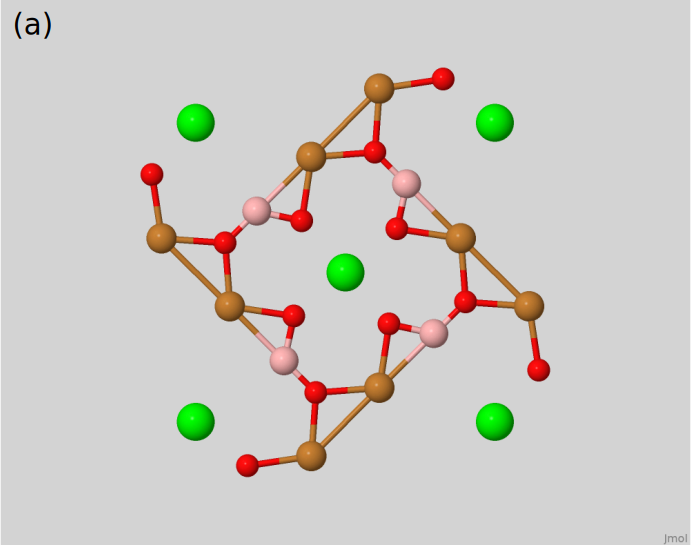
\includegraphics[width=\columnwidth,trim={0 2.5in 0 2.5in},clip]{figures/scbo.pdf}
\end{figure}
\section{Strontium Copper Borate as a Bosonic Topological Insulator}

\section{Low Temperature Thermal Conductivity}


\bibliography{./refs.bib}
\bibliographystyle{unsrt}

\end{document}
